\section{External interface requirements}
\label{sec:external_interface_requirements}%

\subsection{User Interfaces}
\label{subsec:User_interfaces}%

Students, businesses, and university administrators will be able to access the InternHub - Students \& Companies (S\&C) platform's \textbf{user interface} via a \textbf{responsive web application} on any device with a current web browser and an internet connection.
\subsubsection{Authentication Interface}
\begin{enumerate}
    \item User login and registration.
    \item Password reset functionality.
    \item Multi-factor authentication (optional).
\end{enumerate}

\begin{figure}[H]
    \centering
    \begin{minipage}{0.33\textwidth}
        \centering
        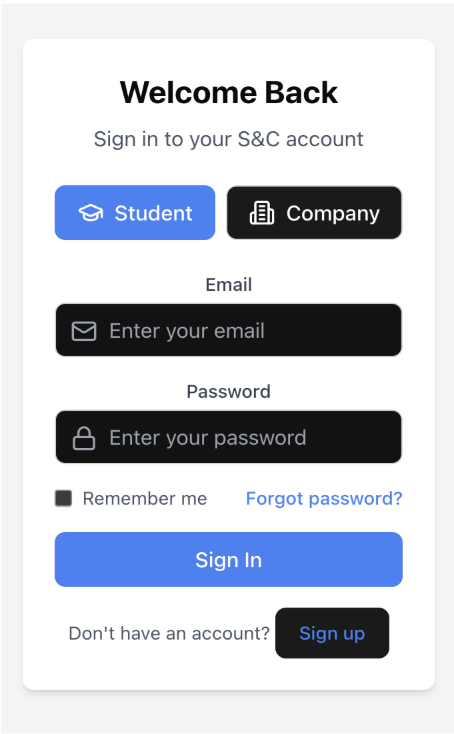
\includegraphics[width=\linewidth]{JhaBhatiaSharma/Images/Mockups/Login.png}
        \caption{Login mockup.}
        \label{fig:login_mockup}
    \end{minipage}
    \hspace{1cm} % Adjust the space between images
    \begin{minipage}{0.33\textwidth}
        \centering
        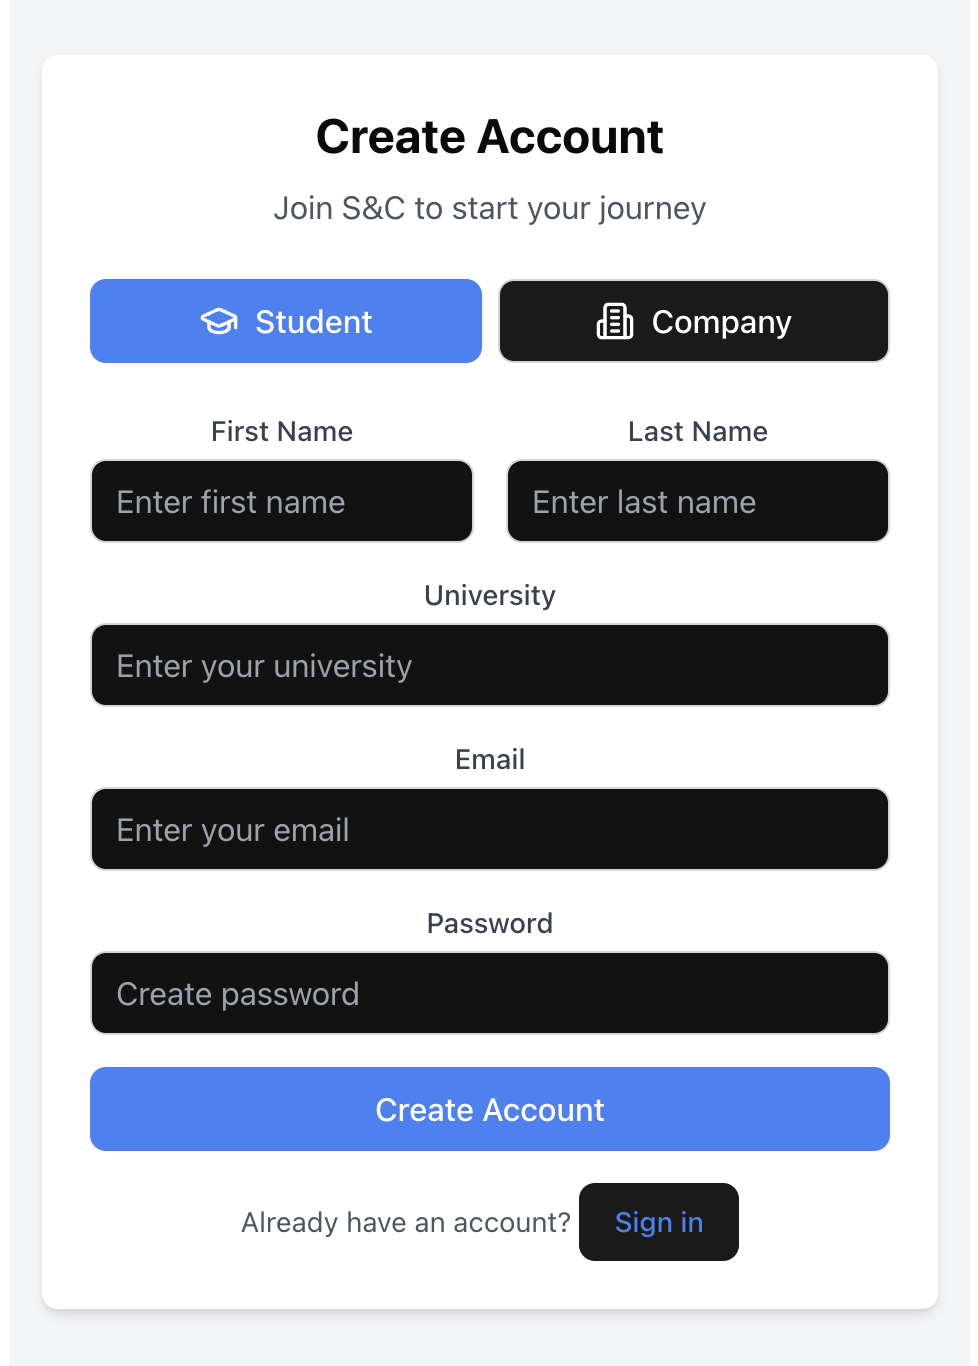
\includegraphics[width=\linewidth]{JhaBhatiaSharma/Images/Mockups/SignUp.png}
        \caption{SignUp mockup.}
        \label{fig:signup_mockup}
    \end{minipage}
\end{figure}



\subsubsection{Student Interface}
\begin{enumerate}
    \item \textbf{Dashboard Overview:} Shows notifications, recommended internships, and active applications.
    \item \textbf{Profile Management:} Add or update qualifications and edit personal information.
    \item \textbf{CV Builder:} Use built-in templates to create and manage resumes.
    \item \textbf{Internship Search:} Look for and select internships according to talents, domain, and location.
    \item \textbf{Application Tracker:} Check the progress of applications that have been submitted.
    \item \textbf{Interview Calendar:} Organize interview dates with the calendar feature.
    \item \textbf{Messaging System:} Interact with administrators and businesses.
\end{enumerate}

\begin{figure}[H]
    \begin{center}
        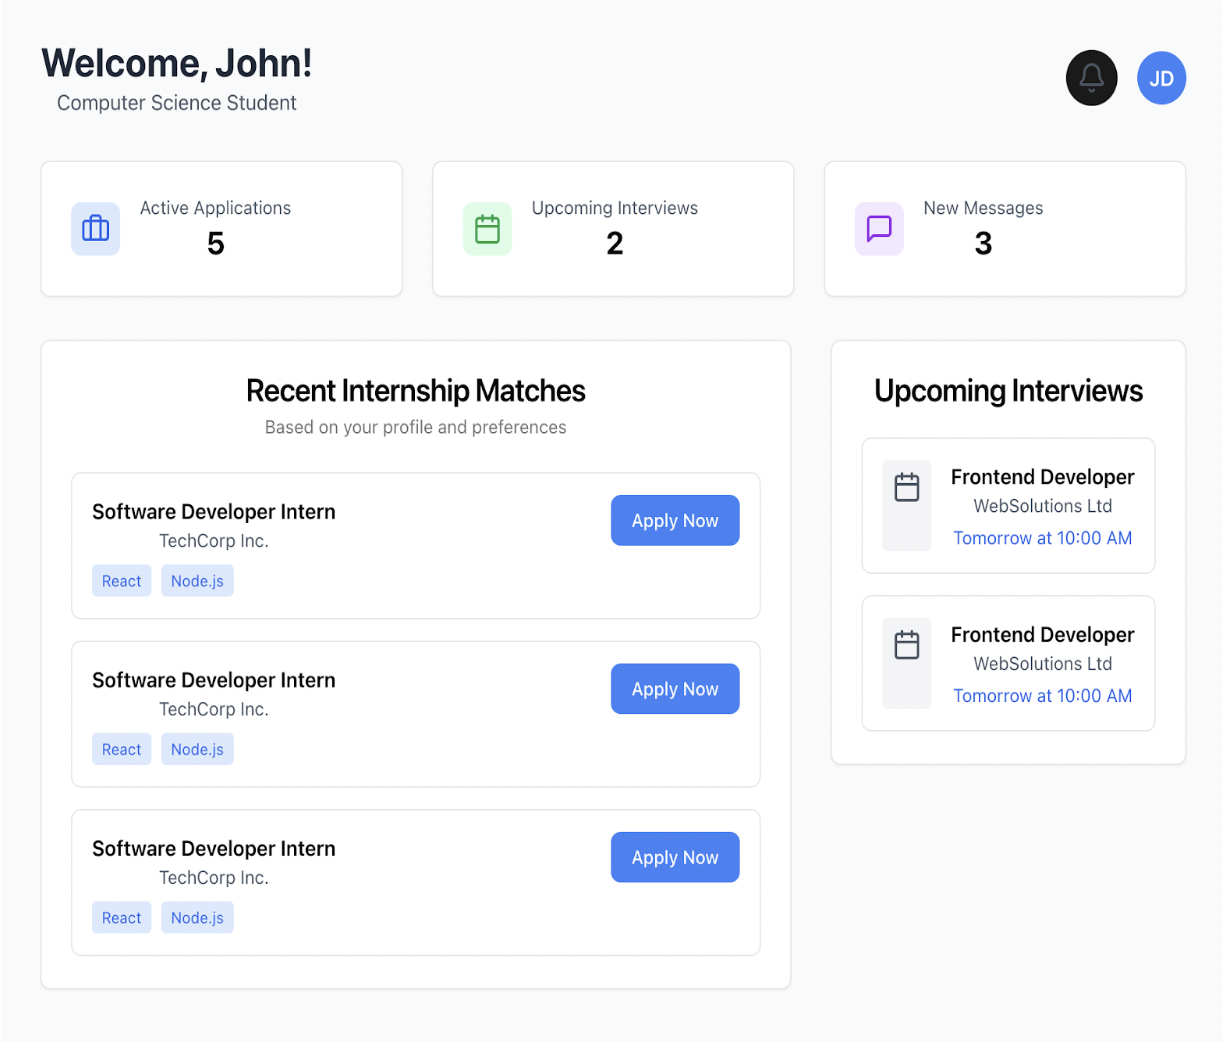
\includegraphics[width=0.82\linewidth]{JhaBhatiaSharma/Images/Mockups/StudentInterface.png}
        \caption{Student Interface Diagram}
        \label{fig:StudentInterface}%
    \end{center}
\end{figure}

\subsubsection{Company Interface}
\begin{enumerate}
    \item \textbf{Dashboard Overview:} Displays applications, postings, and other data.
    \item \textbf{Management of Company Profiles:} Modify logos and company information.
    \item \textbf{Management of Internship Postings:} Produce and oversee internship advertisements.
    \item \textbf{Managing Candidates:} Examine applications and create a shortlist of applicants.
    \item \textbf{Interview Scheduler:} Use a scheduling tool to plan and monitor interviews.
    \item \textbf{Analytics Dashboard:} Access information on posting engagement and candidate performance.
\end{enumerate}

\begin{figure}[H]
    \begin{center}
        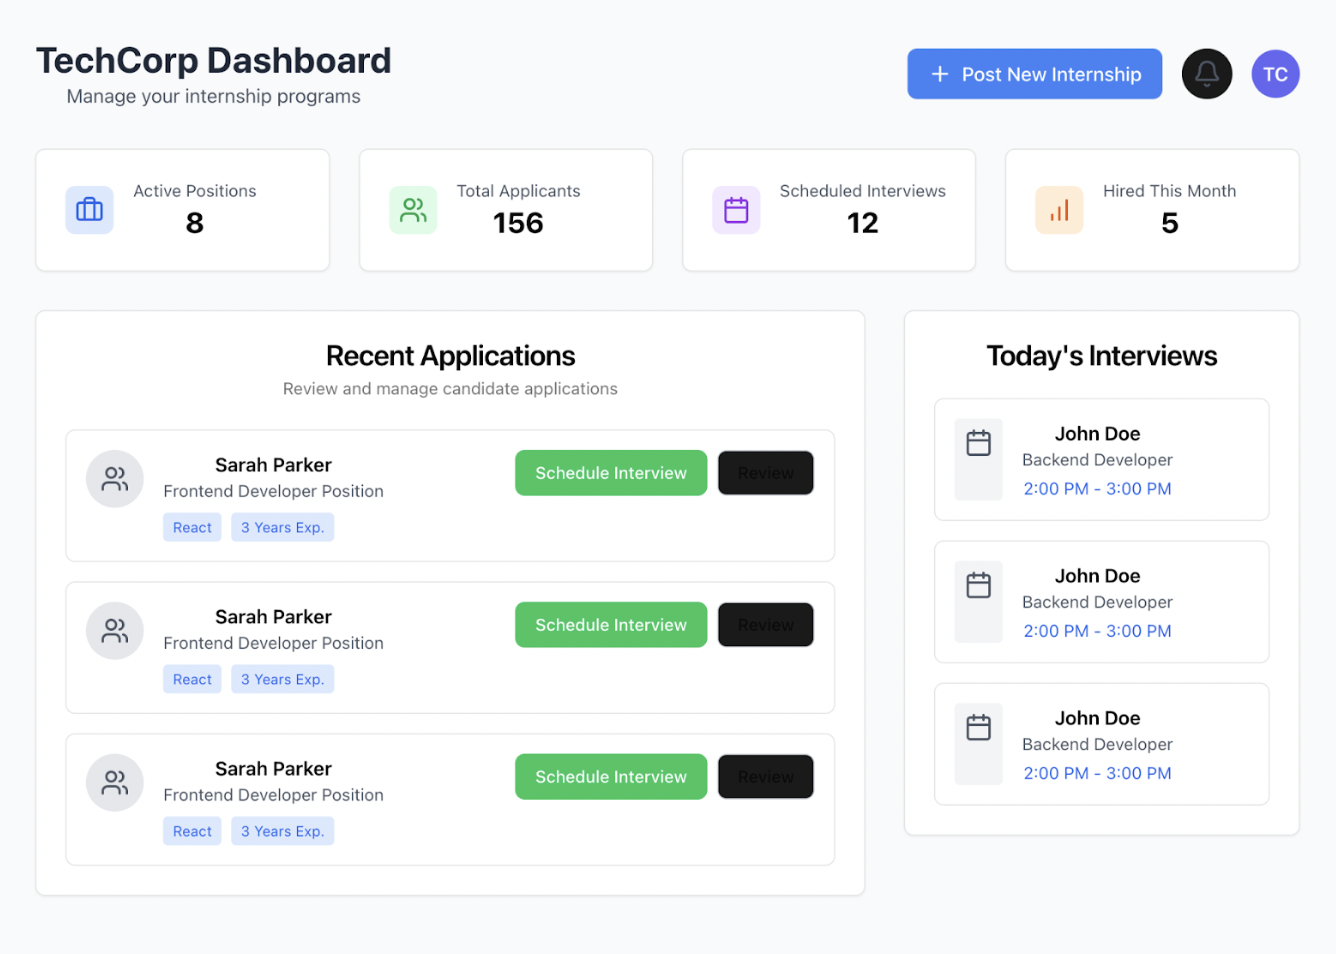
\includegraphics[width=0.82\linewidth]{JhaBhatiaSharma/Images/Mockups/CompanyInterface.png}
        \caption{Company Interface Diagram}
        \label{fig:CompanyInterface}%
    \end{center}
\end{figure}

\subsubsection{Administrator Interface}
\begin{enumerate}
    \item \textbf{System Overview:} Keep an eye on the status and activities of the platform.
    \item \textbf{User Management:} Oversee users, including administrators, businesses, and students.
    \item \textbf{Handling Complaints:} Examine and address complaints that have been submitted.
    \item \textbf{Report Creation:} Produce reports on internship progress and platform usage.
    \item \textbf{Configuration Settings:} Modify settings for the entire system.
\end{enumerate}

\begin{figure}[H]
    \begin{center}
        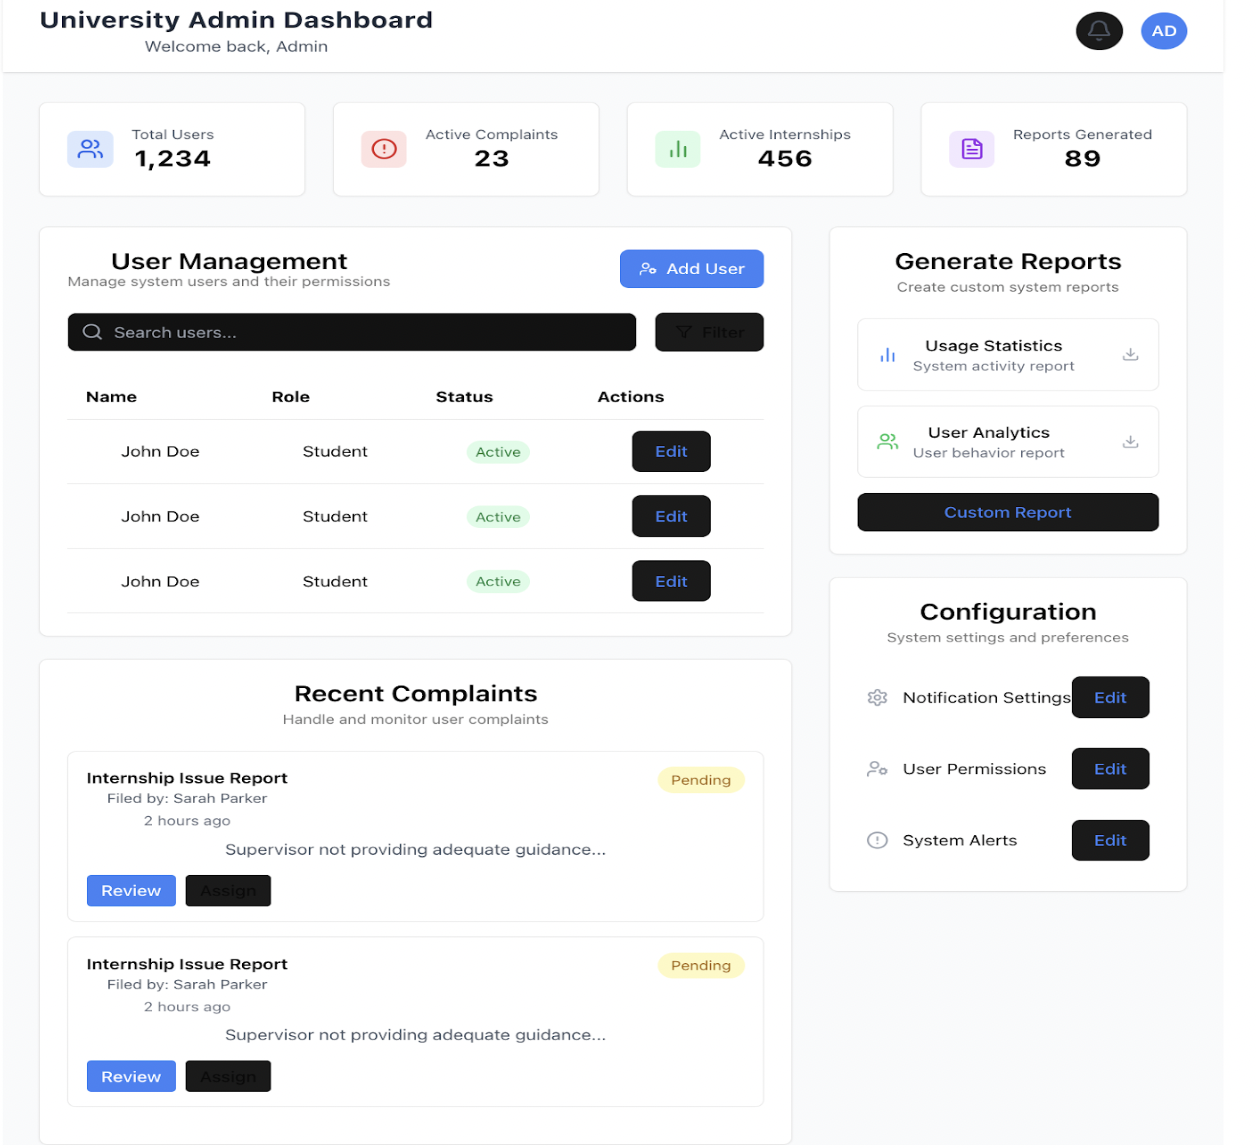
\includegraphics[width=0.82\linewidth]{JhaBhatiaSharma/Images/Mockups/AdminInterface.png}
        \caption{Administrator Interface Diagram}
        \label{fig:AdministratorInterface}%
    \end{center}
\end{figure}

\subsection{Hardware Interfaces}
\label{subsec:hardware_interfaces}%

\begin{itemize}
    \item Compatible with both desktop and mobile web browsers available today.
    \item Minimum screen resolution: 1280x720.
    \item Supports mobile devices with touch interfaces.
    \item Features for uploading and downloading resumes, job descriptions, and feedback files.
\end{itemize}

\subsection{Software Interfaces}
\label{subsec:software_interfaces}%

\begin{itemize}
    \item \textbf{Database Management System:} Stores user information, internships, and system logs.
    \item \textbf{Email Server:} Provides emails for confirmation and notifications.
    \item \textbf{File Storage System:} Manages uploaded documents, including resumes.
    \item \textbf{Authentication System:} Manages role-based access and user login.
    \item \textbf{Analytics Engine:} Produces usage reports and offers insights.
\end{itemize}


\subsection{Communication Interfaces}
\label{subsec:communication_interfaces}%

\begin{itemize}
    \item \textbf{HTTPS Protocol:} Ensures secure communication between users and the platform.
    \item \textbf{RESTful API:} Enables seamless communication between the front-end and back-end systems.
    \item \textbf{WebSocket Connections:} Supports real-time notifications for updates and alerts.
    \item \textbf{Email SMTP:} Manages email correspondence for notifications and alerts.
\end{itemize}

\section{Functional Requirements}
\label{sec:functional_requirements}%

\subsection{Requirements Lists}
\label{subsec:requirements3}%
\newcounter{req}
\setcounter{req}{1}
\newcommand{\creq}{\thereq\stepcounter{req}}

% Functional Requirements for F1
\subsubsection{F1. User Management}
\begin{center}
    \begin{longtable}{ |l|p{0.9\linewidth}| }
        \hline
        \textbf{ID} & \textbf{Description} \\
        \hline
        F1.1 & The system shall allow students, companies, and university administrators to register with verified email addresses. \\
        \hline
        F1.2 & The system shall provide secure authentication with optional two-factor verification. \\
        \hline
        F1.3 & The system shall allow users to update their profile information including contact details and preferences. \\
        \hline
        F1.4 & The system shall enforce role-based access control for students, companies, and administrators. \\
        \hline
        F1.5 & The system shall support password reset functionality with email verification. \\
        \hline
        F1.6 & The system shall maintain audit logs of all user authentication activities. \\
        \hline
        F1.7 & The system shall allow users to manage notification preferences. \\
        \hline
        F1.8 & The system shall enforce strong password policies. \\
        \hline
    \end{longtable}
\end{center}

% Functional Requirements for F2
\subsubsection{F2. CV Management}
\begin{center}
    \begin{longtable}{ |l|p{0.9\linewidth}| }
        \hline
        \textbf{ID} & \textbf{Description} \\
        \hline
        F2.1 & The system shall provide customizable CV templates for students. \\
        \hline
        F2.2 & The system shall allow students to create and store multiple versions of their CVs. \\
        \hline
        F2.3 & The system shall enable students to update their CVs at any time. \\
        \hline
        F2.4 & The system shall allow students to control CV visibility to specific companies. \\
        \hline
        F2.5 & The system shall provide a skill management interface for students. \\
        \hline
        F2.6 & The system shall validate skill entries against a standardized skill database. \\
        \hline
        F2.7 & The system shall support document upload for certificates and portfolios. \\
        \hline
        F2.8 & The system shall track CV view statistics for students. \\
        \hline
    \end{longtable}
\end{center}

% Functional Requirements for F3
\subsubsection{F3. Internship Management}
\begin{center}
    \begin{longtable}{ |l|p{0.9\linewidth}| }
        \hline
        \textbf{ID} & \textbf{Description} \\
        \hline
        F3.1 & The system shall allow companies to create detailed internship postings. \\
        \hline
        F3.2 & The system shall provide an application tracking system for companies. \\
        \hline
        F3.3 & The system shall automatically notify students of application status changes. \\
        \hline
        F3.4 & The system shall provide advanced search and filtering capabilities. \\
        \hline
        F3.5 & The system shall allow companies to set application deadlines. \\
        \hline
        F3.6 & The system shall enable bulk application processing for companies. \\
        \hline
        F3.7 & The system shall support multiple rounds of application review. \\
        \hline
        F3.8 & The system shall maintain a history of all internship postings. \\
        \hline
    \end{longtable}
\end{center}

% Functional Requirements for F4
\subsubsection{F4. Interview Management}
\begin{center}
    \begin{longtable}{ |l|p{0.9\linewidth}| }
        \hline
        \textbf{ID} & \textbf{Description} \\
        \hline
        F4.1 & The system shall provide a calendar interface for interview scheduling. \\
        \hline
        F4.2 & The system shall track interview status and progress. \\
        \hline
        F4.3 & The system shall collect structured feedback from both parties. \\
        \hline
        F4.4 & The system shall send automated interview reminders. \\
        \hline
        F4.5 & The system shall support virtual interview link generation. \\
        \hline
        F4.6 & The system shall allow rescheduling with mutual agreement. \\
        \hline
        F4.7 & The system shall maintain interview history. \\
        \hline
        F4.8 & The system shall support multiple interview rounds. \\
        \hline
    \end{longtable}
\end{center}

% Functional Requirements for F5
\subsubsection{F5. Recommendation System}
\begin{center}
    \begin{longtable}{ |l|p{0.9\linewidth}| }
        \hline
        \textbf{ID} & \textbf{Description} \\
        \hline
        F5.1 & The system shall match students with internships based on skills alignment. \\
        \hline
        F5.2 & The system shall suggest qualified candidates to companies. \\
        \hline
        F5.3 & The system shall learn from user interactions to improve recommendations. \\
        \hline
        F5.4 & The system shall generate personalized internship suggestions. \\
        \hline
        F5.5 & The system shall consider location preferences in matching. \\
        \hline
        F5.6 & The system shall factor in past application success patterns. \\
        \hline
        F5.7 & The system shall update recommendations in real-time. \\
        \hline
        F5.8 & The system shall explain recommendation reasoning to users. \\
        \hline
    \end{longtable}
\end{center}

% Functional Requirements for F6
\subsubsection{F6. Complaint Handling}
\begin{center}
    \begin{longtable}{ |l|p{0.9\linewidth}| }
        \hline
        \textbf{ID} & \textbf{Description} \\
        \hline
        F6.1 & The system shall provide a structured complaint submission interface. \\
        \hline
        F6.2 & The system shall route complaints to appropriate university administrators. \\
        \hline
        F6.3 & The system shall track resolution progress. \\
        \hline
        F6.4 & The system shall support appeals process. \\
        \hline
        F6.5 & The system shall maintain complete complaint history. \\
        \hline
        F6.6 & The system shall enable communication between parties. \\
        \hline
        F6.7 & The system shall generate complaint resolution reports. \\
        \hline
        F6.8 & The system shall enforce resolution timeframes. \\
        \hline
    \end{longtable}
\end{center}

\subsection{Priority and Criticality Matrix}
\label{subsec:priority_criticality_matrix}%

\begin{table}[H]
    \centering
    \begin{tabular}{ |l|l|l|l| }
        \hline
        \textbf{Requirement Category} & \textbf{Priority} & \textbf{Implementation Phase} & \textbf{Criticality} \\
        \hline
        User Management & High & Phase 1 & Critical \\
        \hline
        CV Management & High & Phase 1 & Critical \\
        \hline
        Internship Management & High & Phase 1 & Critical \\
        \hline
        Interview Management & Medium & Phase 2 & Important \\
        \hline
        Recommendation System & Medium & Phase 2 & Important \\
        \hline
        Complaint Handling & Low & Phase 3 & Standard \\
        \hline
    \end{tabular}
    \caption{Priority and Criticality Matrix}
    \label{tab:priority_criticality_matrix}
\end{table}


\subsection{Dependencies}
\label{subsec:dependencies}%

\subsubsection{F1 Dependencies}
\begin{itemize}
    \item \textbf{F1.1:} Must be completed before any other functionality.
    \item \textbf{F1.2:} Is required for all secure operations.
    \item \textbf{F1.4:} Impacts all other functional areas.
\end{itemize}

\subsubsection{F2 Dependencies}
\begin{itemize}
    \item Requires F1 completion.
    \item \textbf{F2.1:} Must be completed before F2.2.
    \item \textbf{F2.5:} Is required for F5.1.
\end{itemize}

\subsubsection{F3 Dependencies}
\begin{itemize}
    \item Requires F1 completion.
    \item \textbf{F3.1:} Must be completed before F3.2.
    \item \textbf{F3.4:} Is required for F5.4.
\end{itemize}

\subsubsection{F4 Dependencies}
\begin{itemize}
    \item Requires F1 and F3 completion.
    \item \textbf{F4.1:} Must be completed before F4.2.
    \item \textbf{F4.3:} Feeds into F5.3.
\end{itemize}

\subsubsection{F5 Dependencies}
\begin{itemize}
    \item Requires F2 and F3 completion.
    \item \textbf{F5.1:} Must be completed before F5.4.
    \item Requires continuous data from F4.3.
\end{itemize}

\subsubsection{F6 Dependencies}
\begin{itemize}
    \item Requires all other systems to be operational.
    \item \textbf{F6.1:} Must be completed before F6.2.
    \item \textbf{F6.4:} Requires F6.3 completion.
\end{itemize}

\newpage
\subsection{Use case diagrams}
\label{subsec:use_case_diagrams}%


\begin{figure}[H]
    \begin{center}
        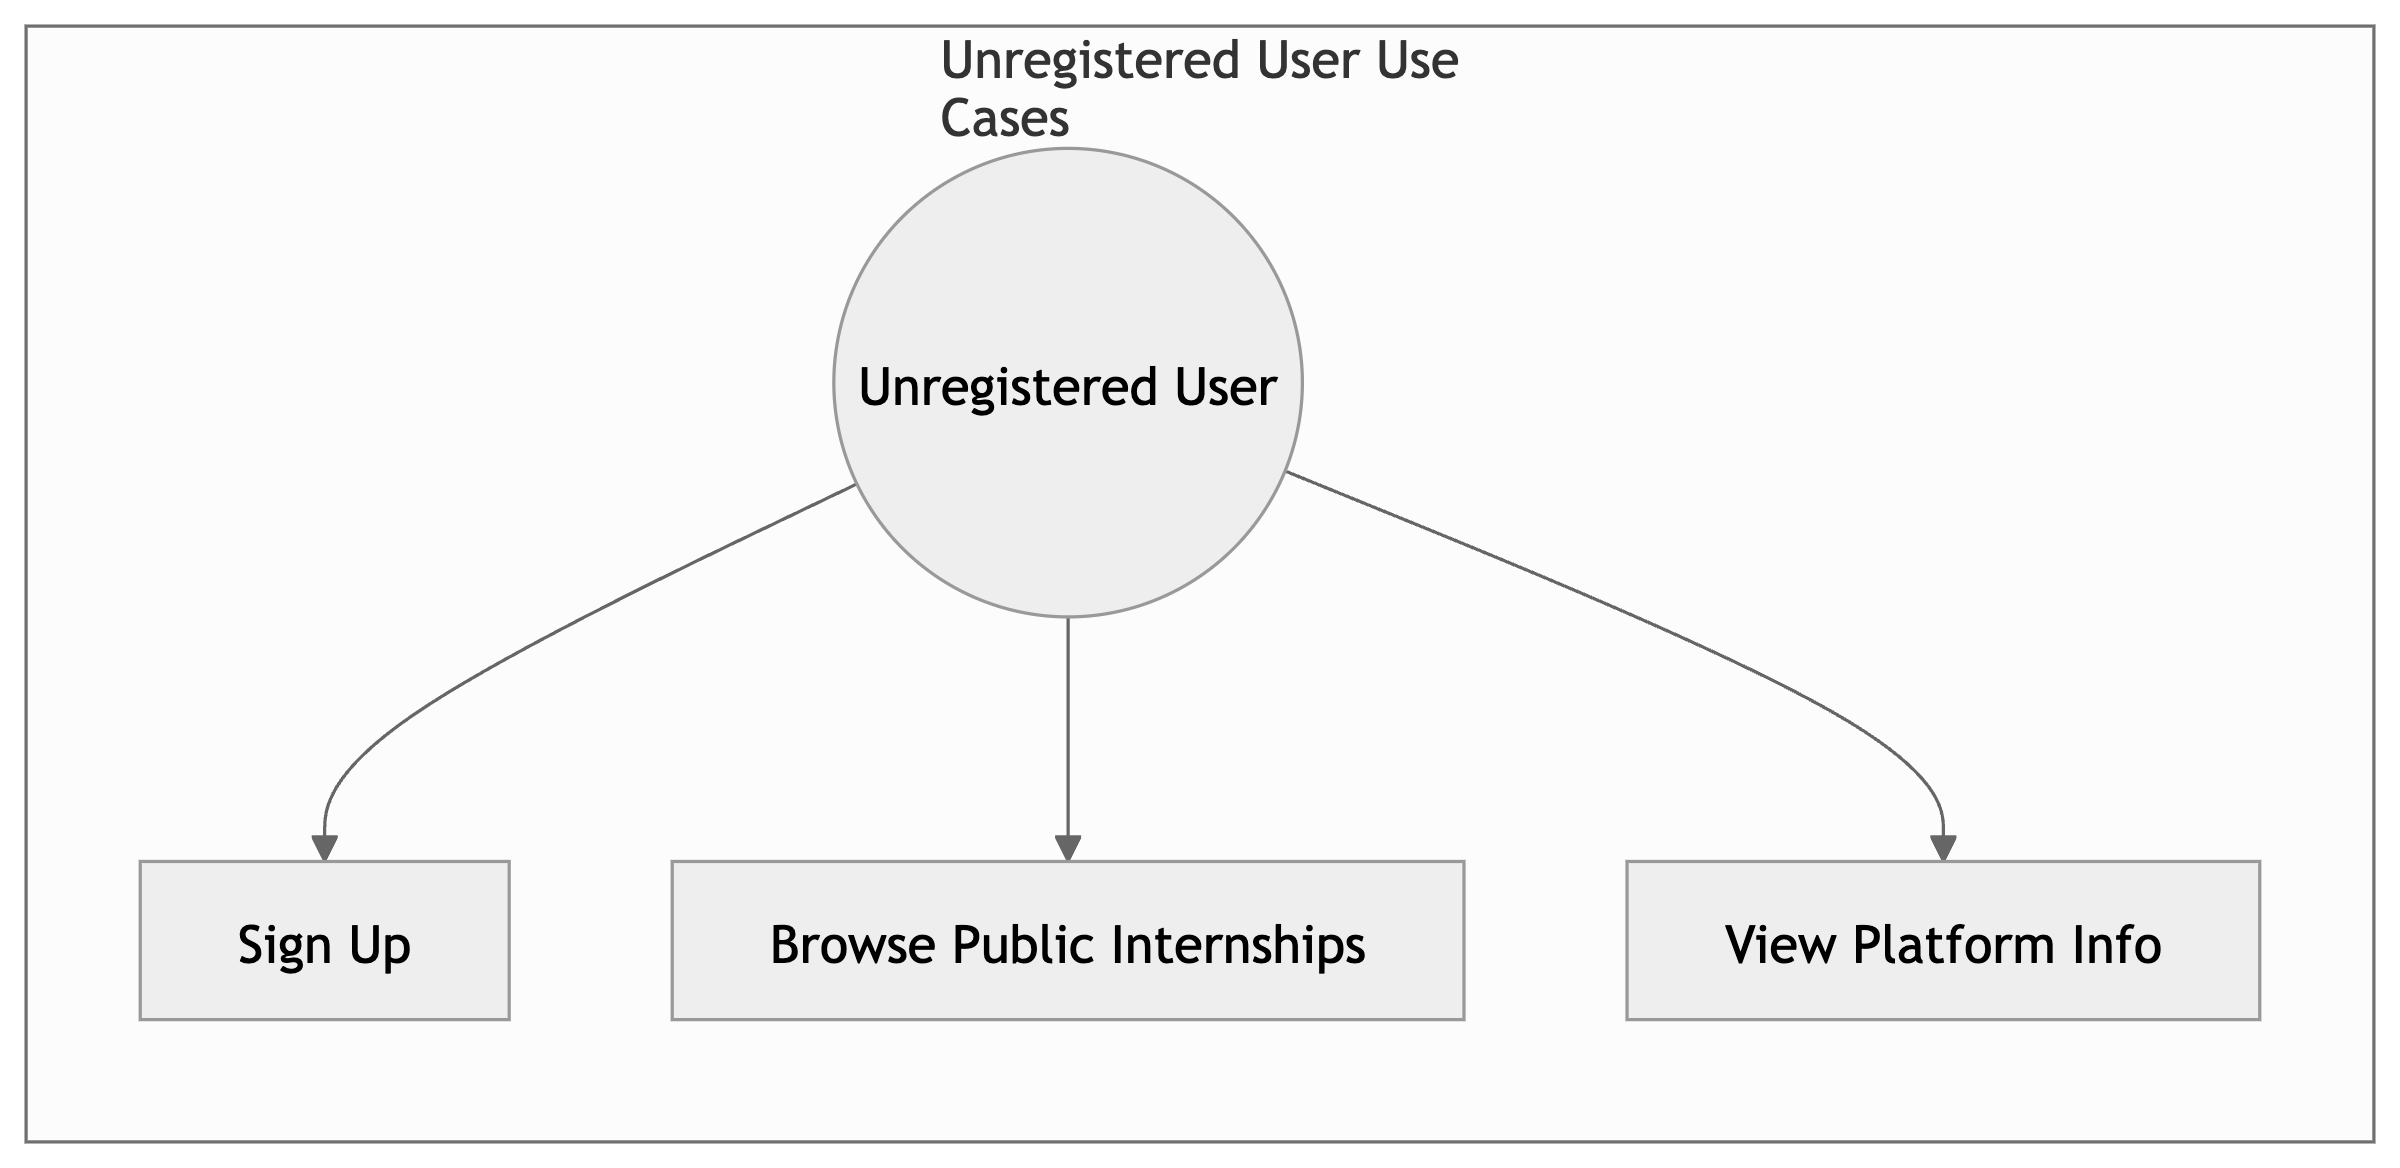
\includegraphics[width=1\linewidth]{JhaBhatiaSharma/Images/Use Case Diagrams/UnregisteredUser.png}
        \caption{Use Cases Diagram for Unregistered Users.} 
        \label{fig:UnregisteredUC}%
    \end{center}
\end{figure}



\begin{figure}[H]
    \begin{center}
        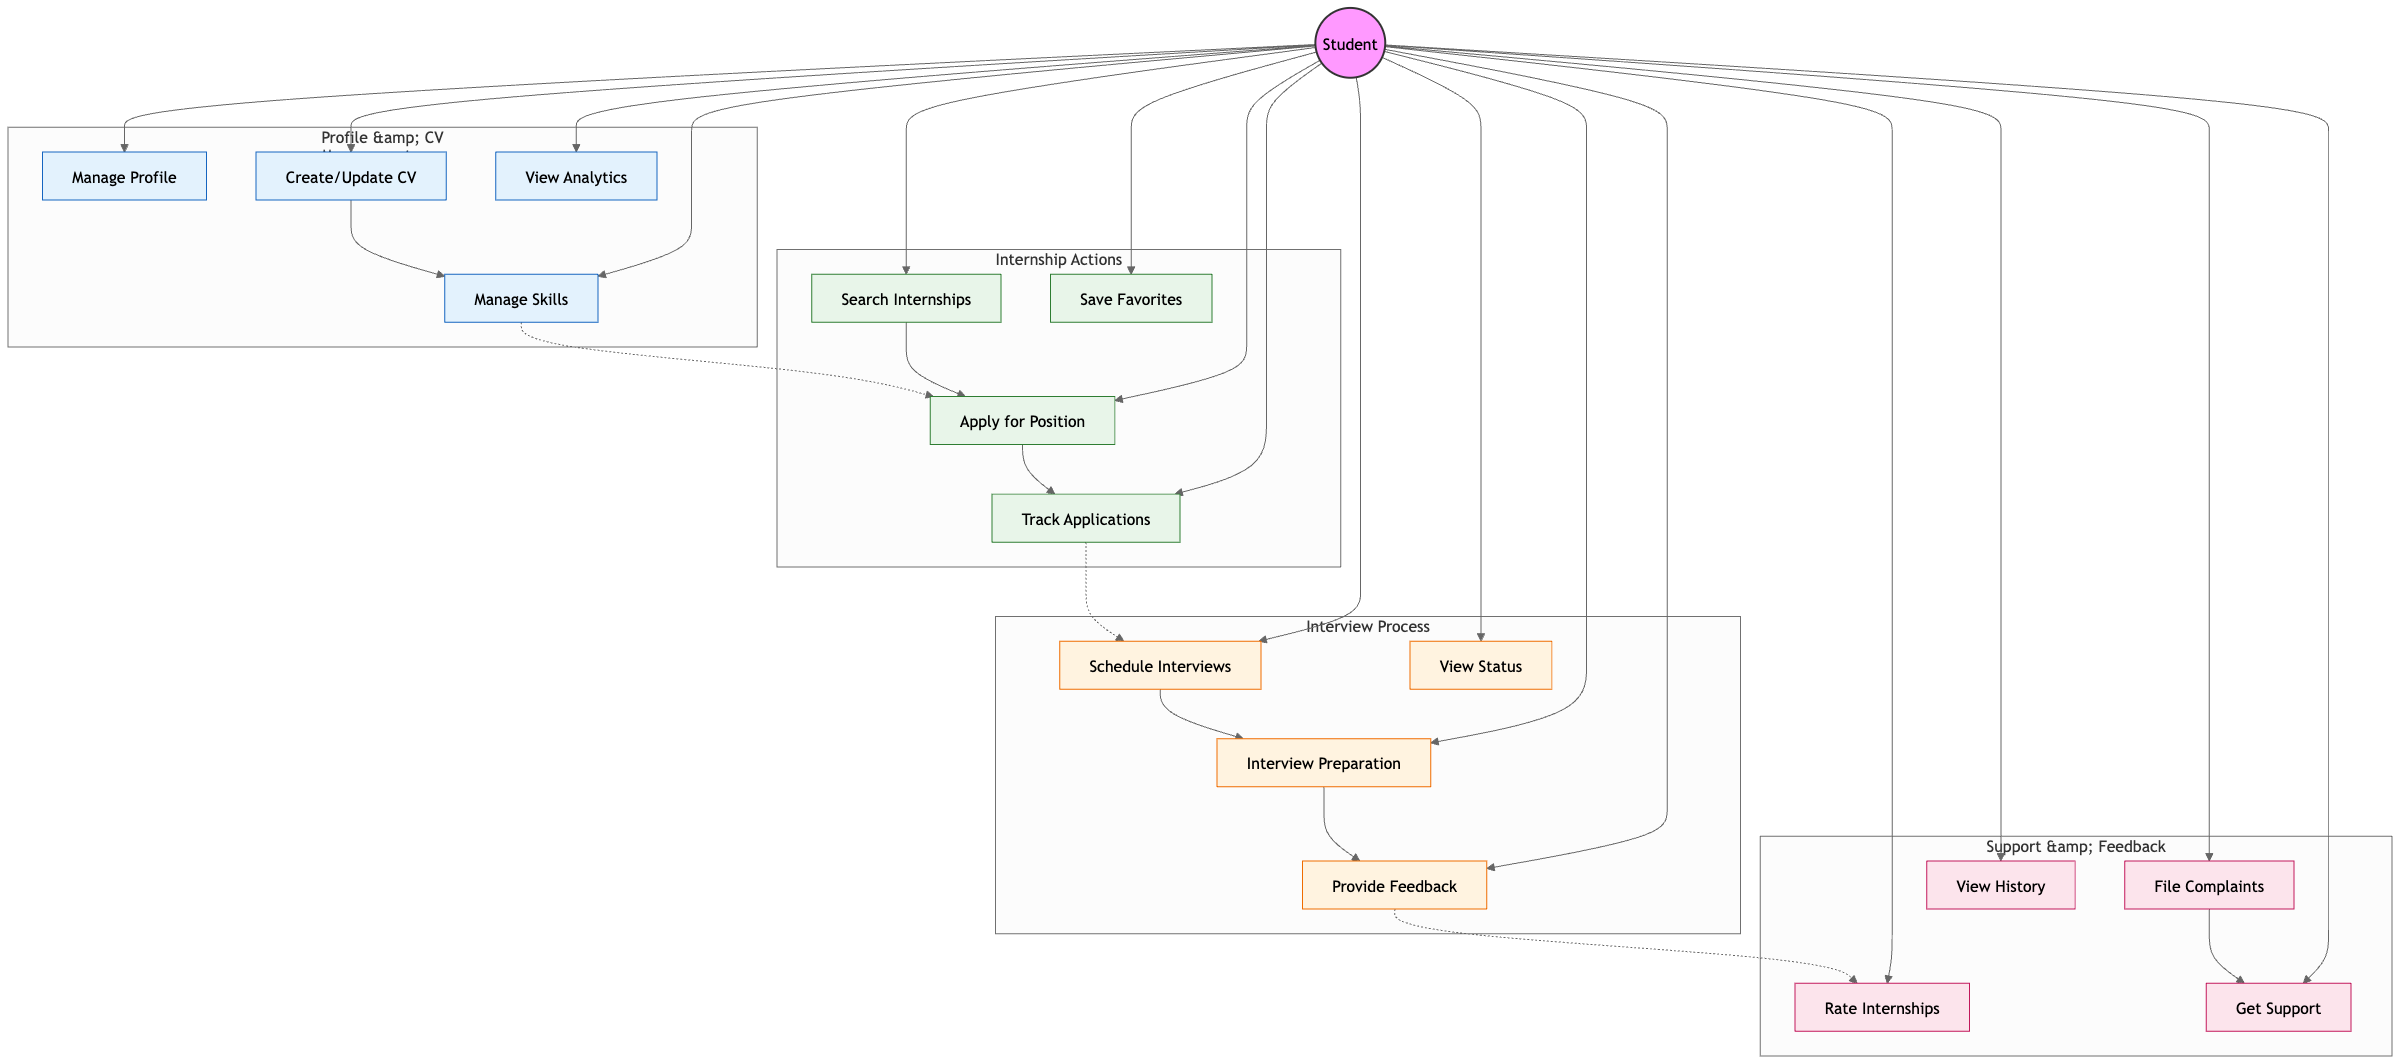
\includegraphics[width=1.15\linewidth]{JhaBhatiaSharma/Images/Use Case Diagrams/Student.png}
        \caption{Use Cases Diagram for Students}
        \label{fig:EducatorUC}%
    \end{center}
\end{figure}



\begin{figure}[H]
    \begin{center}
        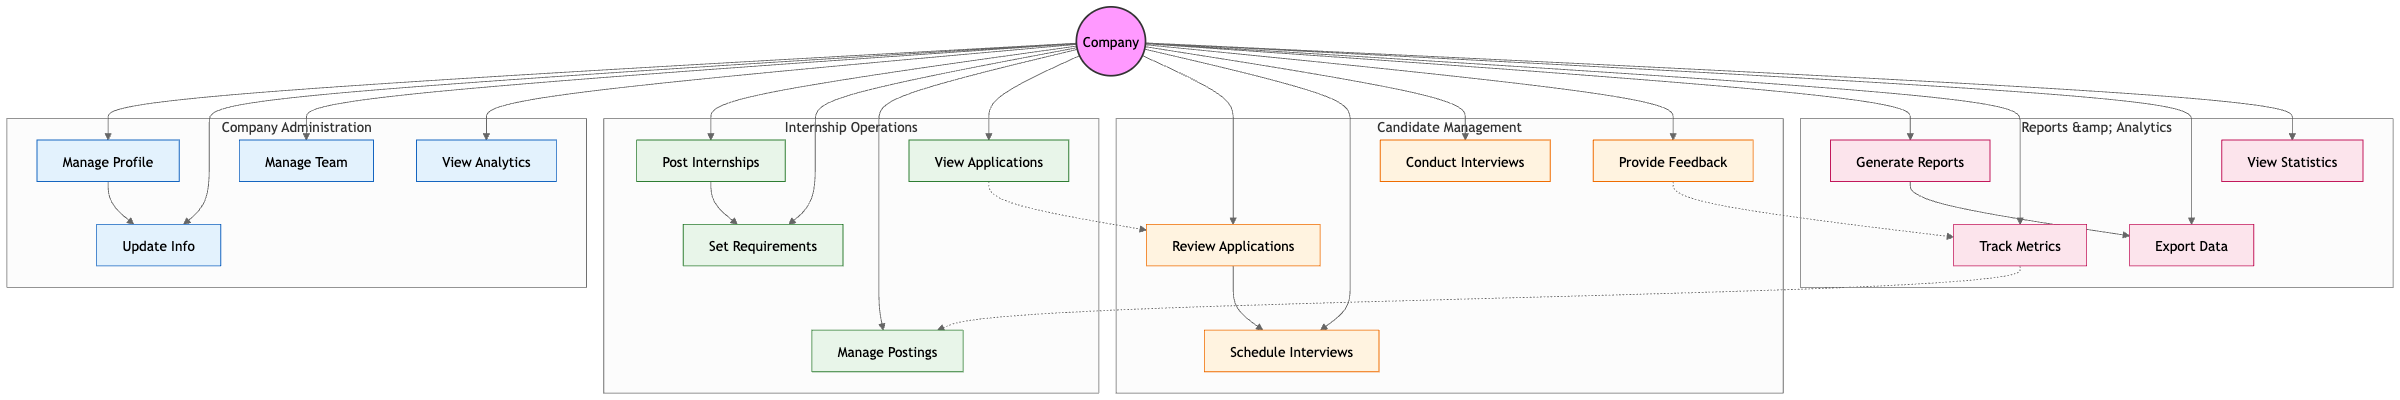
\includegraphics[width=\dimexpr\paperwidth-2cm\relax, height=4cm]{JhaBhatiaSharma/Images/Use Case Diagrams/Company.png}
        \caption{Use Cases Diagram for Companies.}
        \label{fig:CompanyUC}%
    \end{center}
\end{figure}

\begin{figure}[H]
    \begin{center}
        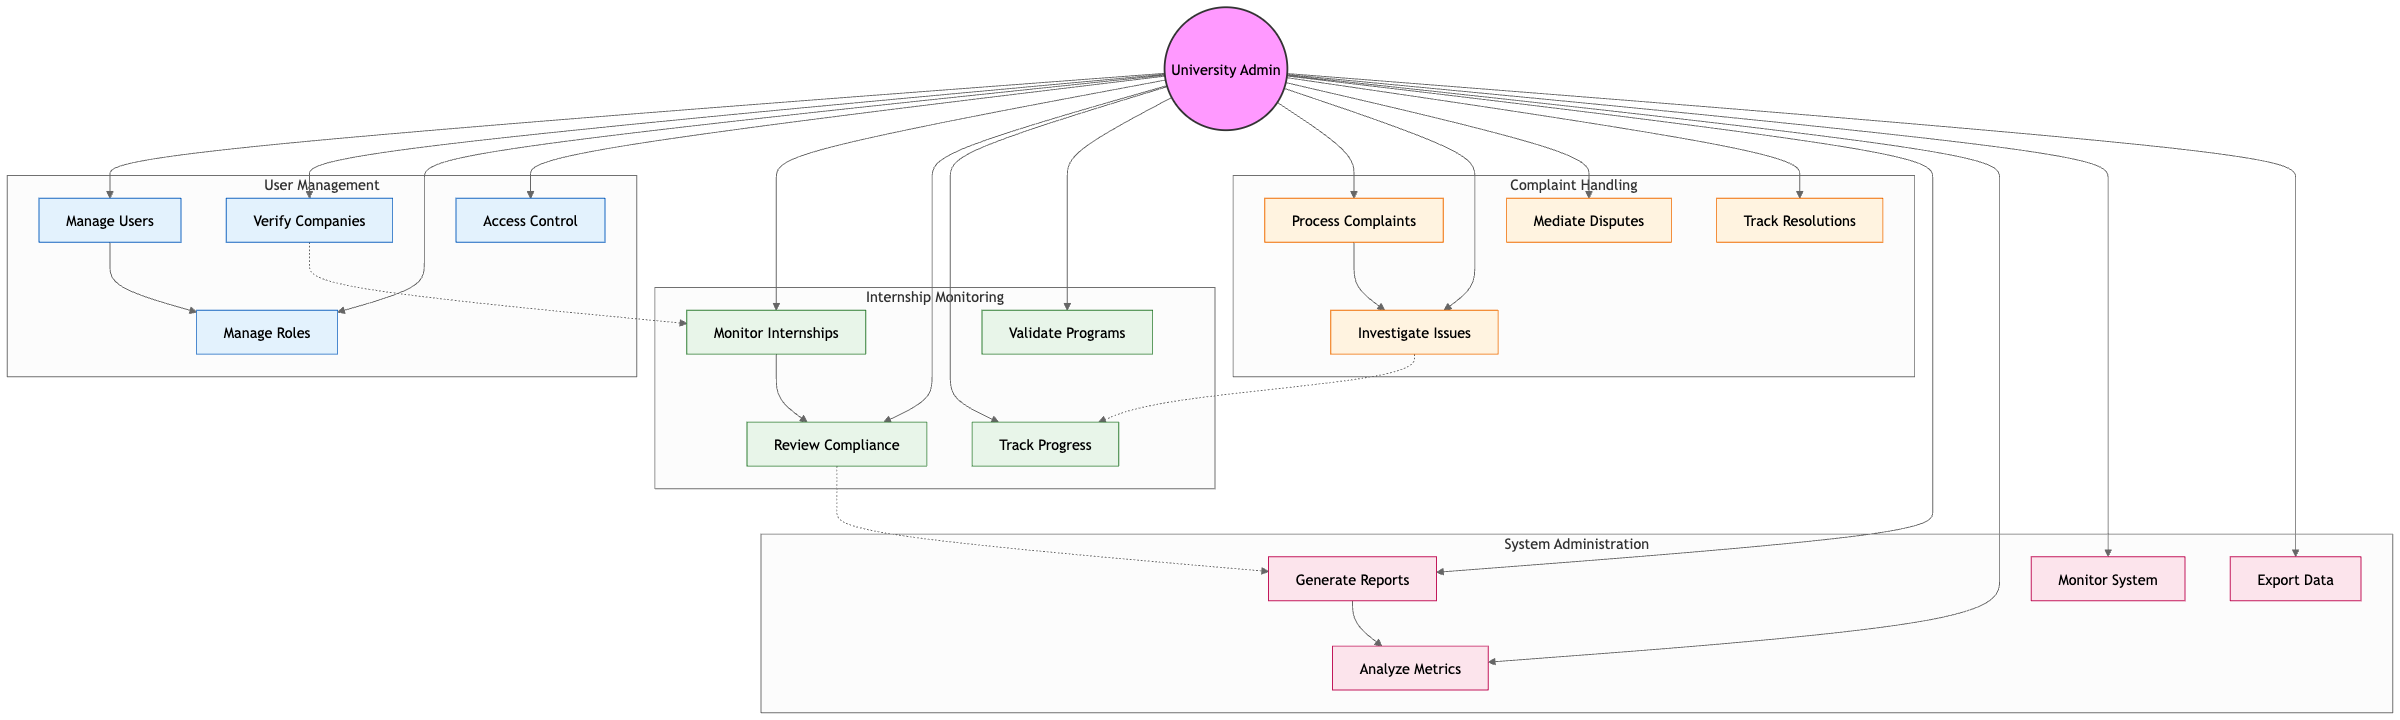
\includegraphics[width=1.1\linewidth, height=4cm]{JhaBhatiaSharma/Images/Use Case Diagrams/Admin.png}
        \caption{Use Cases Diagram for University Admin.}
        \label{fig:AdminUC}%
    \end{center}
\end{figure}

\subsection{Use cases}
\label{subsec: use_cases}%
\newcounter{uc}
\setcounter{uc}{1}
\newcommand{\cuc}{\theuc\stepcounter{uc}}
The primary identified use cases are described and illustrated in this section.
Each of them has a table with \textbf{entry conditions, event row, exit conditions, and exceptions, as well as a sequence diagram} that displays the messages sent back and forth between the called functions and the entities.

\subsubsection*{UC\cuc . Student Registration}
\begin{center}
    \begin{longtable}{|l|p{0.75\linewidth}|}
        \hline
        \textbf{Actor}            & Company Representative, Email Provider \\
        \hline
        \textbf{Entry Conditions} & 
        \begin{itemize}
            \item Company not registered in S\&C
            \item Representative has company email domain
            \item Company meets platform requirements
        \end{itemize} \\
        \hline
        \textbf{Event Flow}       & 
        \begin{enumerate}
            \item S\&C shows the login form with registration option
            \item Representative clicks on "Create Account"
            \item S\&C displays registration form
            \item Representative selects "Register as Company"
            \item Representative enters initial information:
            \begin{itemize}
                \item Company Name
                \item Company Website
                \item Industry Type
                \item Company Size
                \item Company Email Domain
                \item Representative Name
                \item Representative Position
                \item Password
            \end{itemize}
            \item S\&C validates company information
            \item S\&C performs preliminary company verification:
            \begin{itemize}
                \item Website domain matches email domain
                \item Company exists in business registry (if applicable)
            \end{itemize}
            \item S\&C sends verification email
            \item Representative clicks verification link
            \item S\&C prompts for detailed company information:
            \begin{itemize}
                \item Company Description
                \item Office Locations
                \item Logo Upload
                \item Required Documents
            \end{itemize}
            \item S\&C sends information for admin verification
            \item Admin reviews and approves company
            \item S\&C activates company account
            \item S\&C guides through internship posting process
        \end{enumerate} \\
        \hline
        \textbf{Exit Conditions}   & 
        \begin{itemize}
            \item Company account is created and verified
            \item Company profile is complete
            \item Company can post internships
        \end{itemize} \\
        \hline
        \textbf{Exceptions}       & 
        \begin{enumerate}
            \item \textbf{Company already registered:}
            \begin{itemize}
                \item Show existing company message
                \item Provide contact for account recovery
            \end{itemize}
            \item \textbf{Invalid company email domain:}
            \begin{itemize}
                \item Request valid company email
                \item Provide business verification alternatives
            \end{itemize}
            \item \textbf{Company verification failed:}
            \begin{itemize}
                \item Request additional verification documents
                \item Provide support contact
            \end{itemize}
            \item \textbf{Admin rejection:}
            \begin{itemize}
                \item Notify reason for rejection
                \item Provide appeal process information
            \end{itemize}
            \item \textbf{Incomplete required documents:}
            \begin{itemize}
                \item List missing documents
                \item Save partial progress
                \item Allow later completion
            \end{itemize}
        \end{enumerate} \\
        \hline
        \caption{Student Registration Use Case.}
        \label{tab:student_registration_use_case}
    \end{longtable}
\end{center}

\begin{figure}[H]
    \begin{center}
        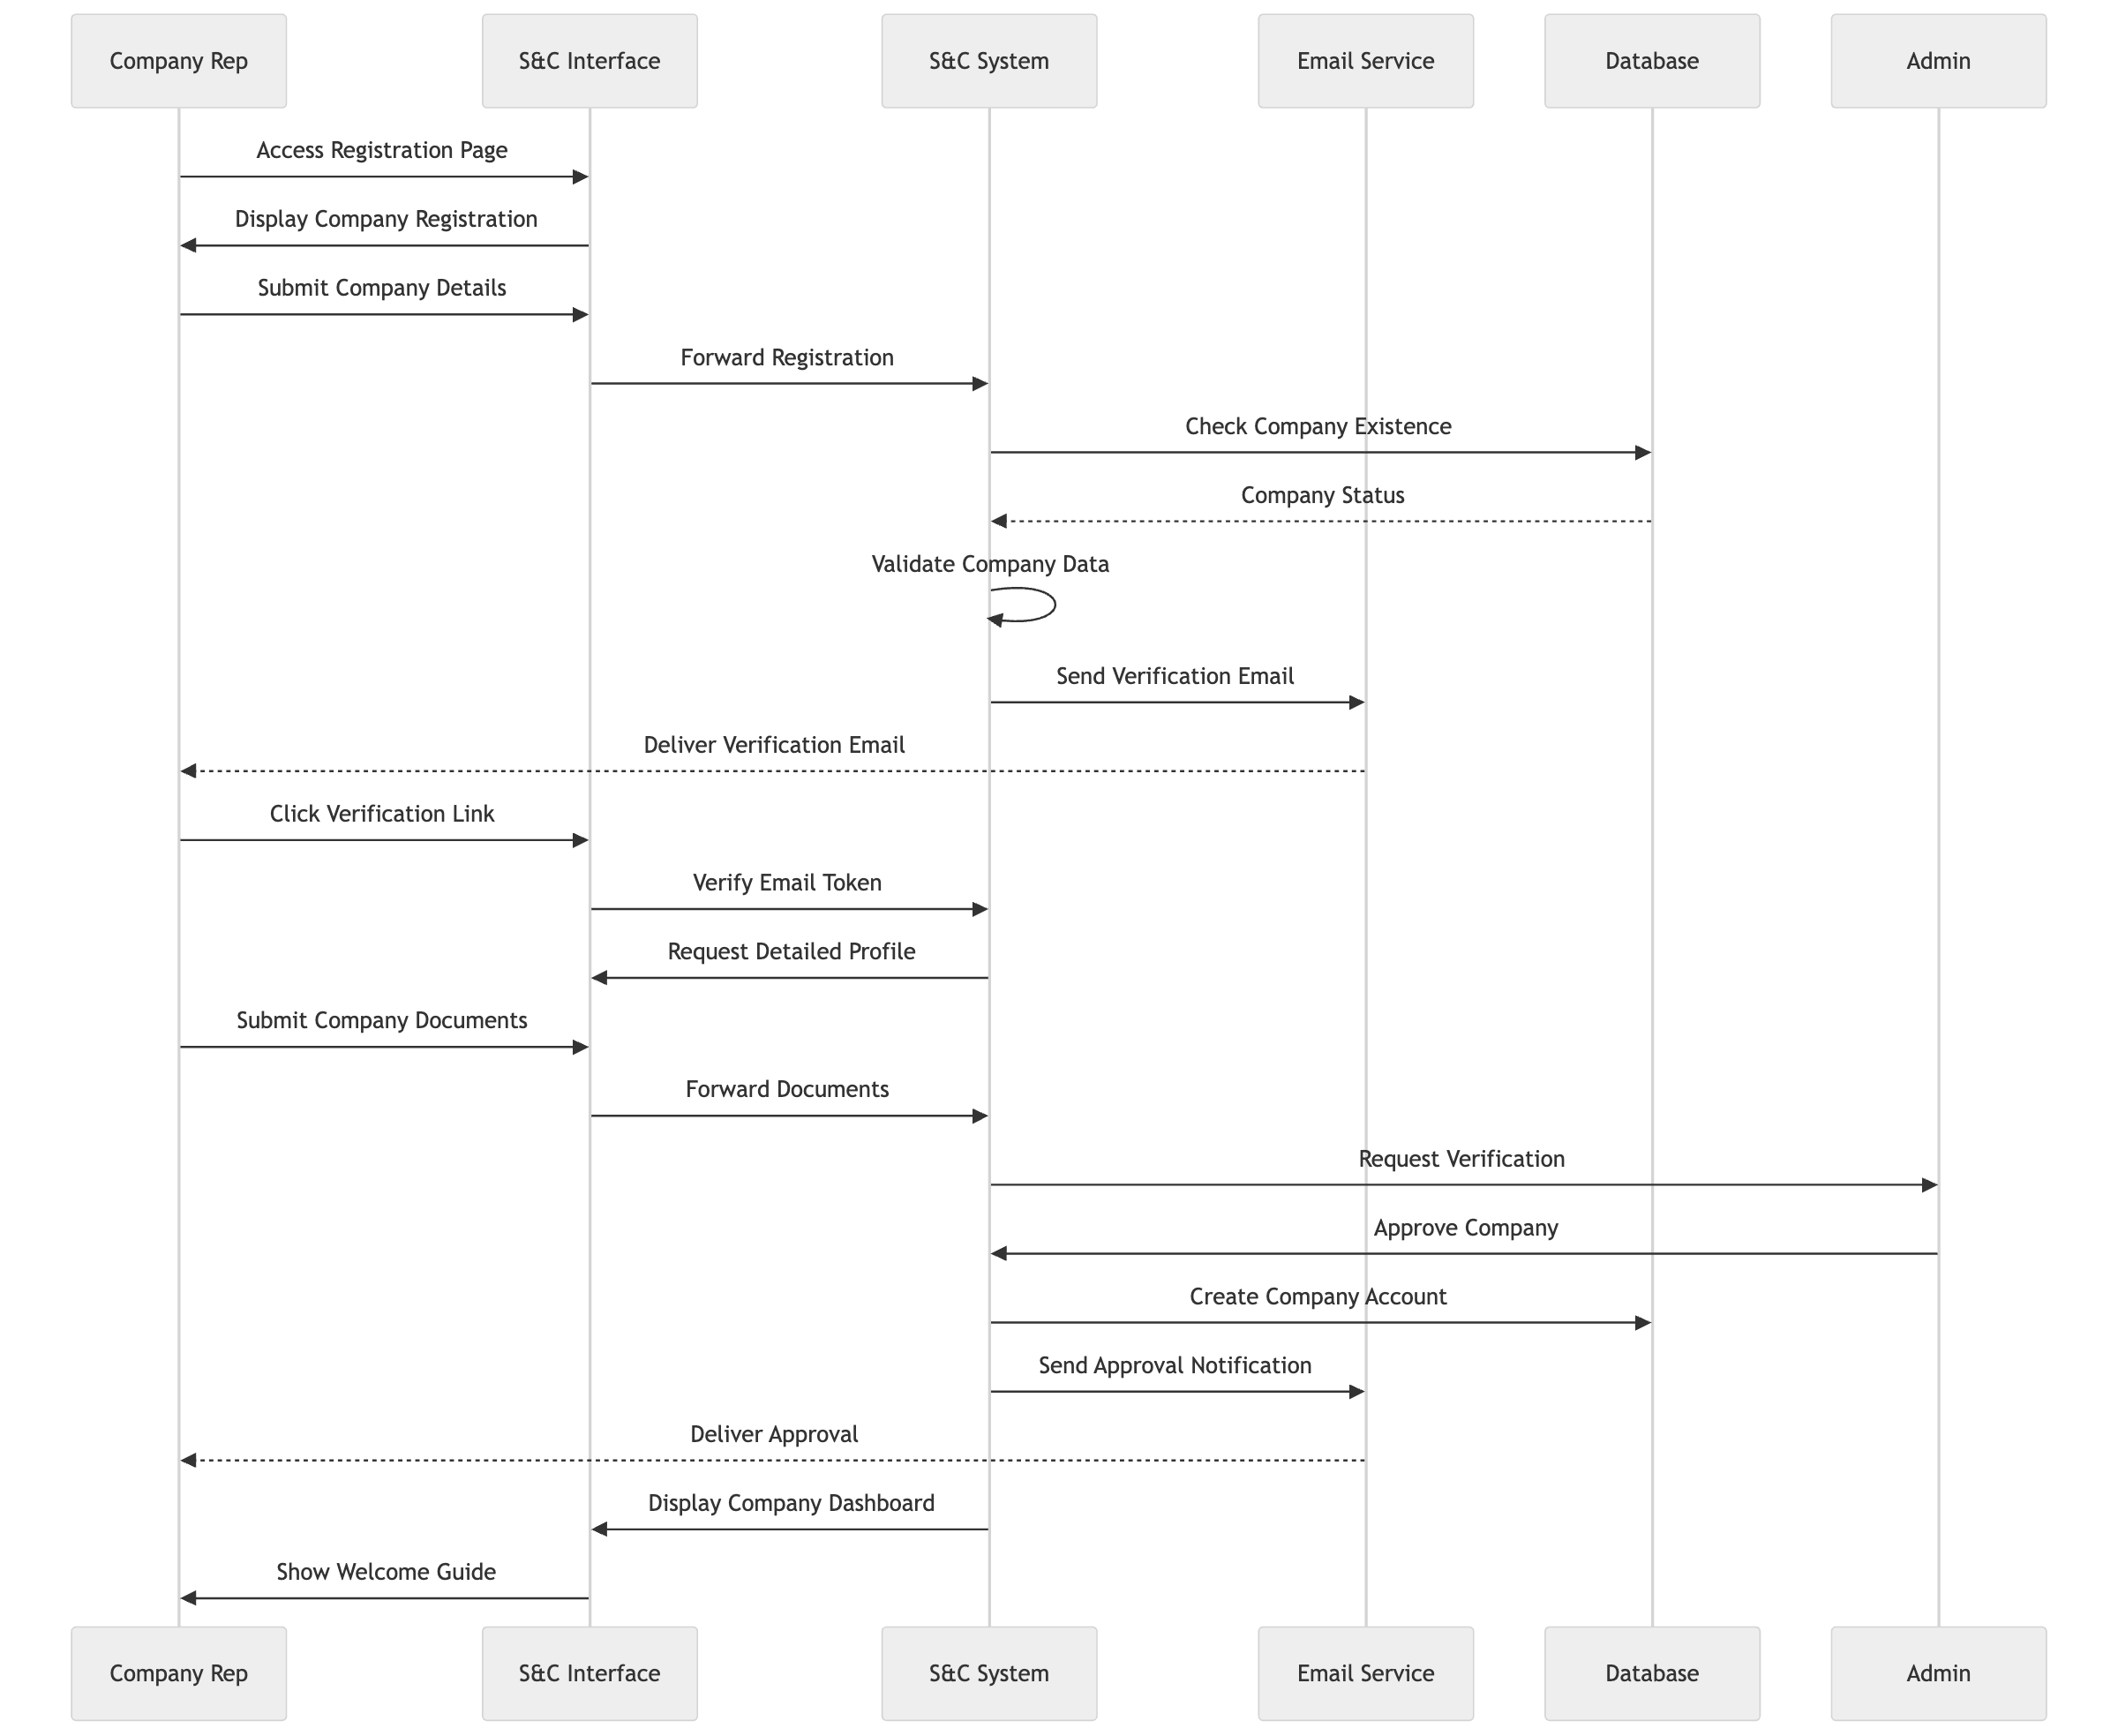
\includegraphics[width=1.15\linewidth, height=\paperheight, keepaspectratio=true]{JhaBhatiaSharma/Images/Sequence Diagrams/StudentRegistration.png}
        \caption{Sequence Diagram for Student Registration}
        \label{fig:signup_as_ED_seqd}%
    \end{center}
\end{figure}

\subsubsection*{UC\cuc . Company Registration}
\begin{center}
    \begin{longtable}{|l|p{0.75\linewidth}|}
        \hline
        \textbf{Actor}            & Company Representative, Email Provider \\
        \hline
        \textbf{Entry Conditions} & 
        \begin{itemize}
            \item Company not registered in S\&C
            \item Representative has company email domain
            \item Company meets platform requirements
        \end{itemize} \\
        \hline
        \textbf{Event Flow}       & 
        \begin{enumerate}
            \item S\&C shows the login form with registration option.
            \item Representative clicks on "Create Account".
            \item S\&C displays registration form.
            \item Representative selects "Register as Company".
            \item Representative enters initial information:
            \begin{itemize}
                \item Company Name
                \item Company Website
                \item Industry Type
                \item Company Size
                \item Company Email Domain
                \item Representative Name
                \item Representative Position
                \item Password
            \end{itemize}
            \item S\&C validates company information.
            \item S\&C performs preliminary company verification:
            \begin{itemize}
                \item Website domain matches email domain
                \item Company exists in business registry (if applicable)
            \end{itemize}
            \item S\&C sends verification email.
            \item Representative clicks verification link.
            \item S\&C prompts for detailed company information:
            \begin{itemize}
                \item Company Description
                \item Office Locations
                \item Logo Upload
                \item Required Documents
            \end{itemize}
            \item S\&C sends information for admin verification.
            \item Admin reviews and approves company.
            \item S\&C activates company account.
            \item S\&C guides through internship posting process.
        \end{enumerate} \\
        \hline
        \textbf{Exit Conditions}   & 
        \begin{itemize}
            \item Company account is created and verified.
            \item Company profile is complete.
            \item Company can post internships.
        \end{itemize} \\
        \hline
        \textbf{Exceptions}       & 
        \begin{enumerate}
            \item \textbf{Company already registered:}
            \begin{itemize}
                \item Show existing company message.
                \item Provide contact for account recovery.
            \end{itemize} 
            \item \textbf{Invalid company email domain:} \begin{itemize}
                \item Request valid company email.
                \item Provide business verification alternatives.
            \end{itemize} 
            \item \textbf{Company verification failed:} \begin{itemize}
                \item Request additional verification documents.
                \item Provide support contact.
            \end{itemize} 
            \item \textbf{Admin rejection:} 
            \begin{itemize}
                \item Notify reason for rejection.
                \item Provide appeal process information.
            \end{itemize} 
            \item \textbf{Incomplete required documents:} \begin{itemize}
                \item List missing documents.
                \item Save partial progress.
                \item Allow later completion.
            \end{itemize}  
        \end{enumerate} \\
        \hline
        \caption{Company Registration use case.}
        \label{tab:company_registration_use_case}
    \end{longtable}
\end{center}


\begin{figure}[H]
    \begin{center}
        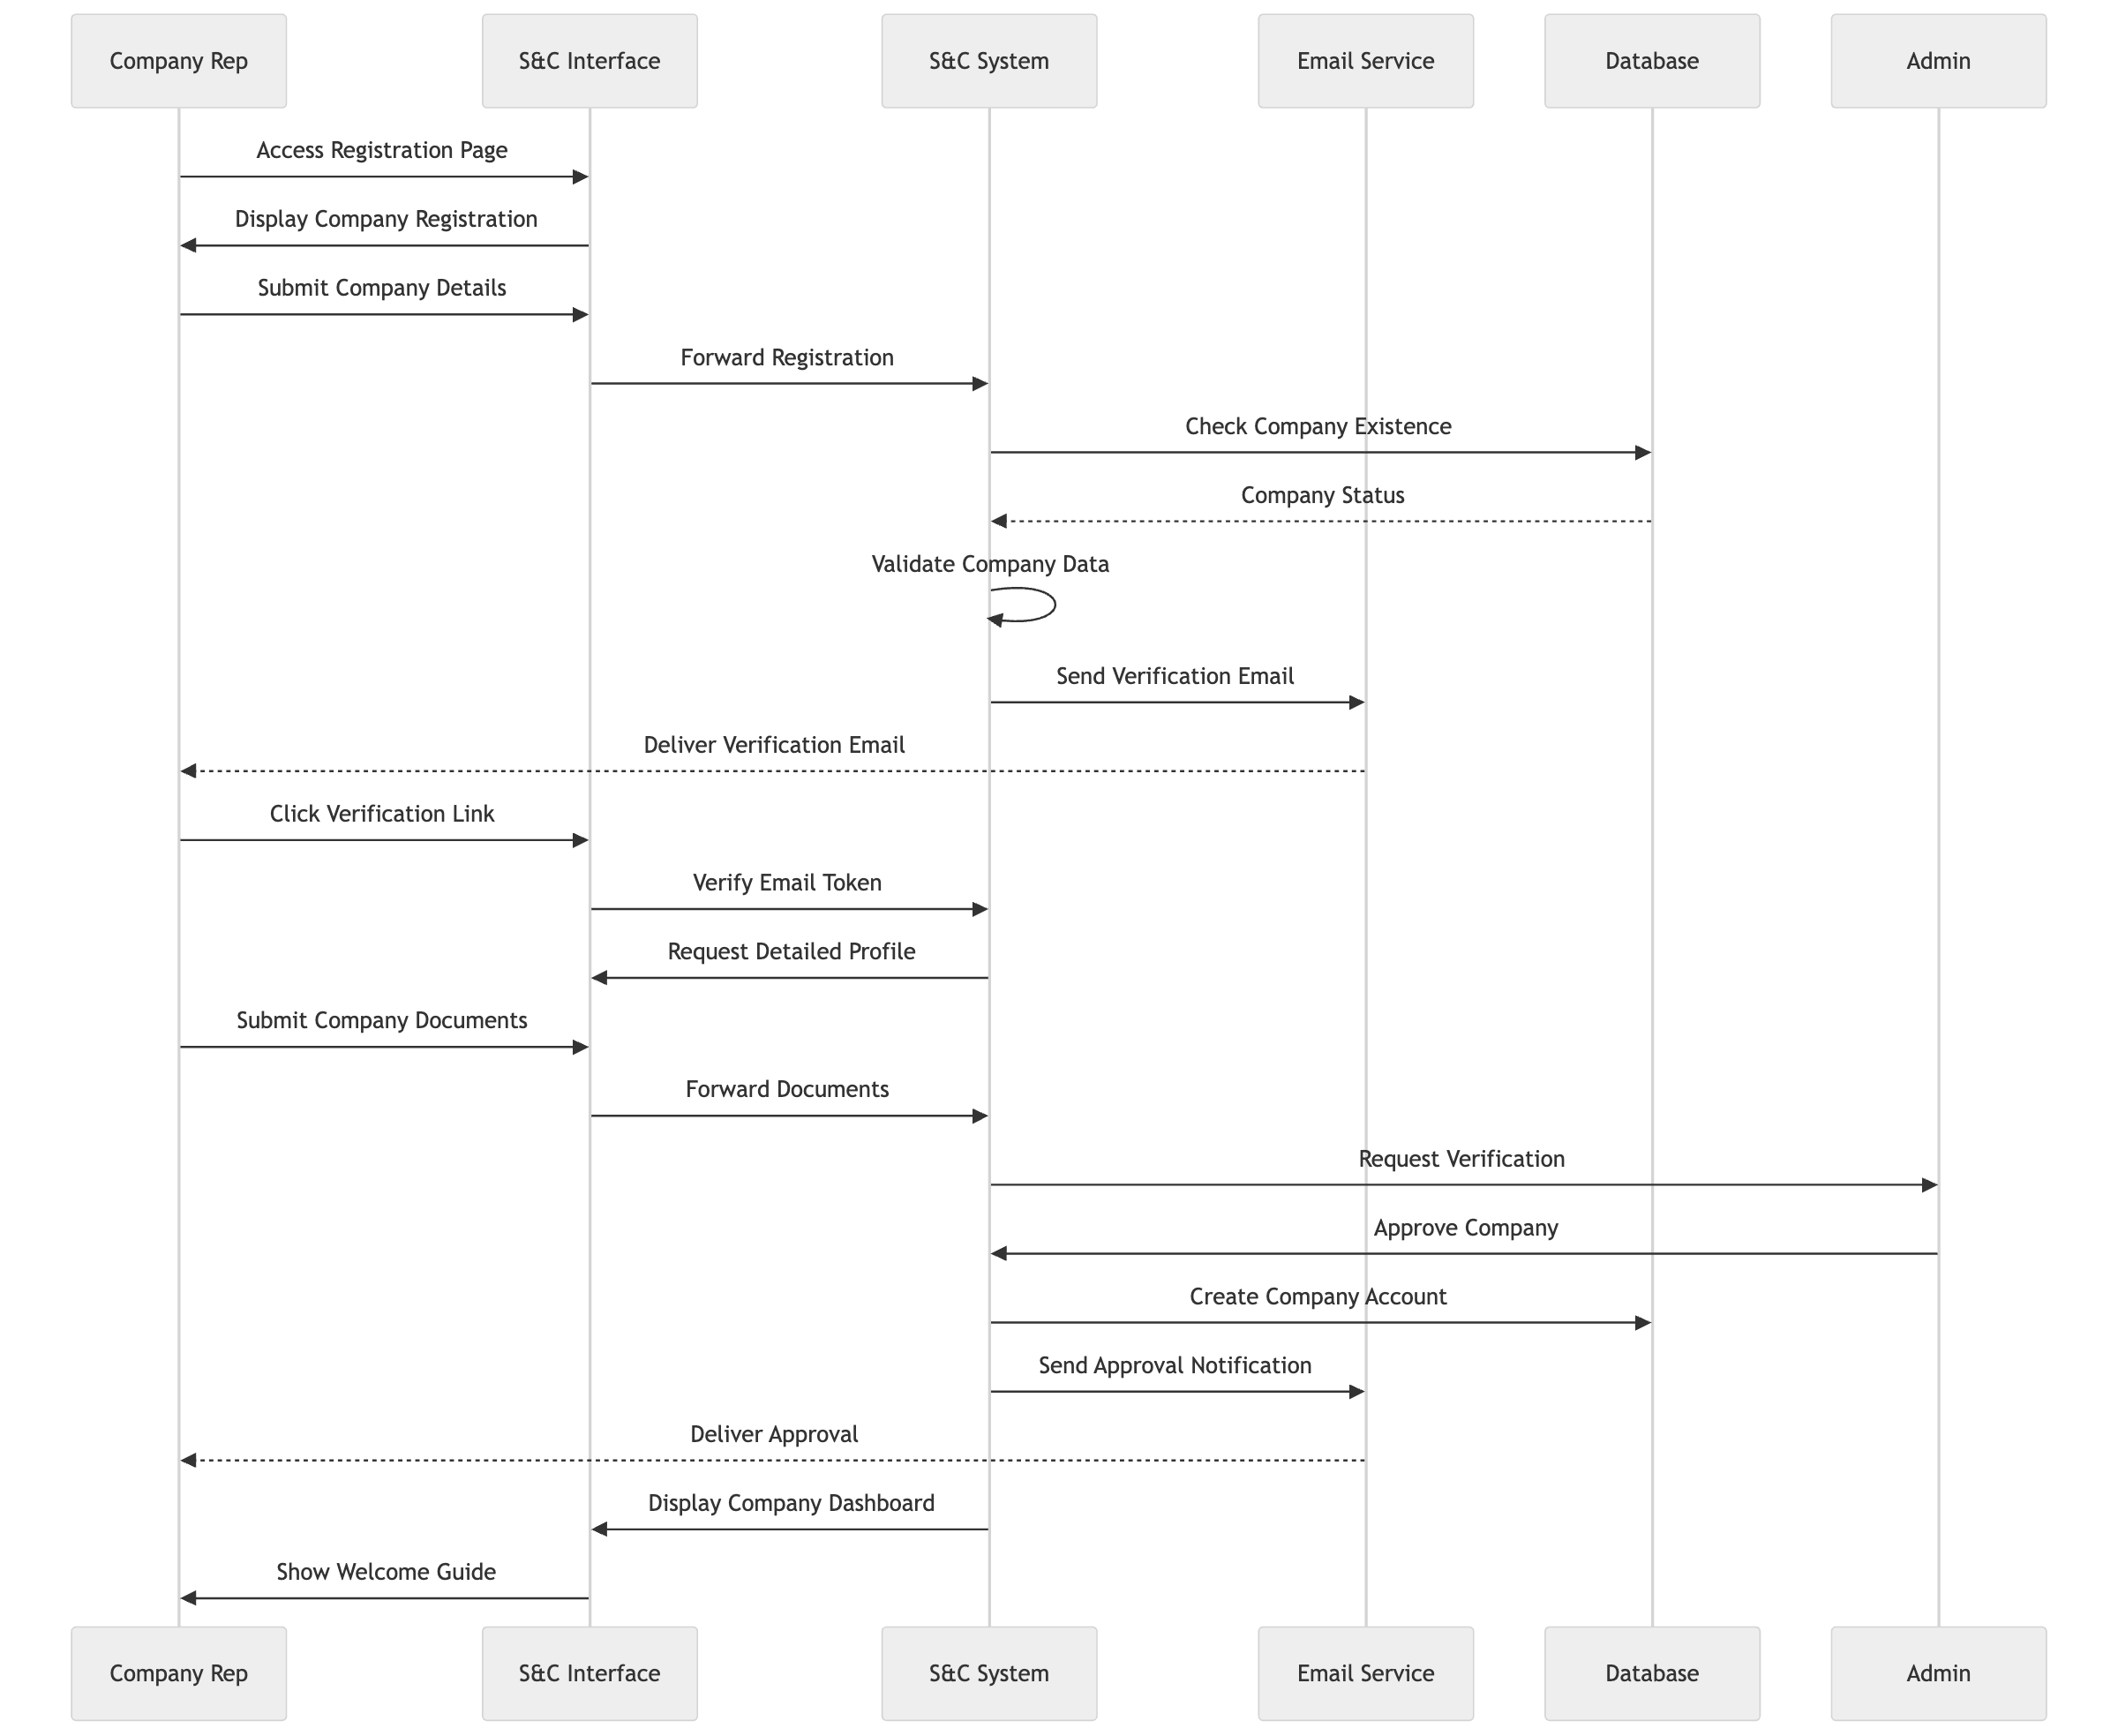
\includegraphics[width=1\linewidth]{JhaBhatiaSharma/Images/Sequence Diagrams/CompanyRegistration.png}
        \caption{Sequence Diagram for Company Registration}
        \label{fig:signup_as_ST_seqd}%
    \end{center}
\end{figure}

\subsubsection*{UC\cuc . Internship Posting}
\begin{center}
    \begin{longtable}{|l|p{0.75\linewidth}|}
        \hline
        \textbf{Actor}            & Company Representative \\
        \hline
        \textbf{Entry Conditions} & 
        \begin{itemize}
            \item Company is verified and logged in
            \item Company profile is complete
            \item Company has posting privileges
        \end{itemize} \\
        \hline
        \textbf{Event Flow}       & 
        \begin{enumerate}
            \item Company accesses internship management dashboard.
            \item Clicks "Post New Internship" button.
            \item S\&C displays internship creation form.
            \item Company enters internship details:
            \begin{itemize}
                \item Position Title
                \item Department
                \item Duration
                \item Start Date
                \item Required Skills
                \item Preferred Skills
                \item Educational Requirements
                \item Responsibilities
                \item Compensation Details
                \item Application Deadline
                \item Number of Positions
                \item Location/Remote Status
            \end{itemize}
            \item Company sets additional preferences:
            \begin{itemize}
                \item Interview Process Steps
                \item Required Documents
                \item Assessment Criteria
            \end{itemize}
            \item S\&C validates all input fields.
            \item Company previews posting.
            \item Company submits for review.
            \item S\&C performs automated checks:
            \begin{itemize}
                \item Content appropriateness
                \item Completeness
                \item Compliance with platform rules
            \end{itemize}
            \item S\&C processes posting:
            \begin{itemize}
                \item Indexes for search
                \item Matches with student profiles
                \item Generates recommendations
            \end{itemize}
            \item S\&C activates posting.
            \item Notifies matching students.
        \end{enumerate} \\
        \hline
        \textbf{Exit Conditions}   & 
        \begin{itemize}
            \item Internship is posted and visible
            \item Matching students are notified
            \item Position appears in search results
        \end{itemize} \\
        \hline
        \textbf{Exceptions}       & 
        \begin{enumerate}
            \item \textbf{Incomplete Required Fields:} \begin{itemize}
                \item Highlight missing fields.
                \item Save as draft.
            \end{itemize} 
            \item \textbf{Invalid Date Combinations:} 
            \begin{itemize}
                \item Show date validation error.
                \item Suggest valid date ranges.
            \end{itemize} 
            \item \textbf{Non-Compliant Content:} 
            \begin{itemize}
                \item Flag specific issues.
                \item Provide compliance guidelines.
            \end{itemize} 
            \item \textbf{Duplicate Posting:} 
            \begin{itemize}
                \item Show existing posting.
                \item Offer update option.
            \end{itemize} 
            \item \textbf{Posting Limit Reached:} 
            \begin{itemize}
                \item Show upgrade options.
                \item Manage existing posts.
            \end{itemize} 
        \end{enumerate} \\
        \hline
        \caption{Internship Posting Use Case.}
        \label{tab:internship_posting_use_case}
    \end{longtable}
\end{center}

\begin{figure}[H]
    \begin{center}
        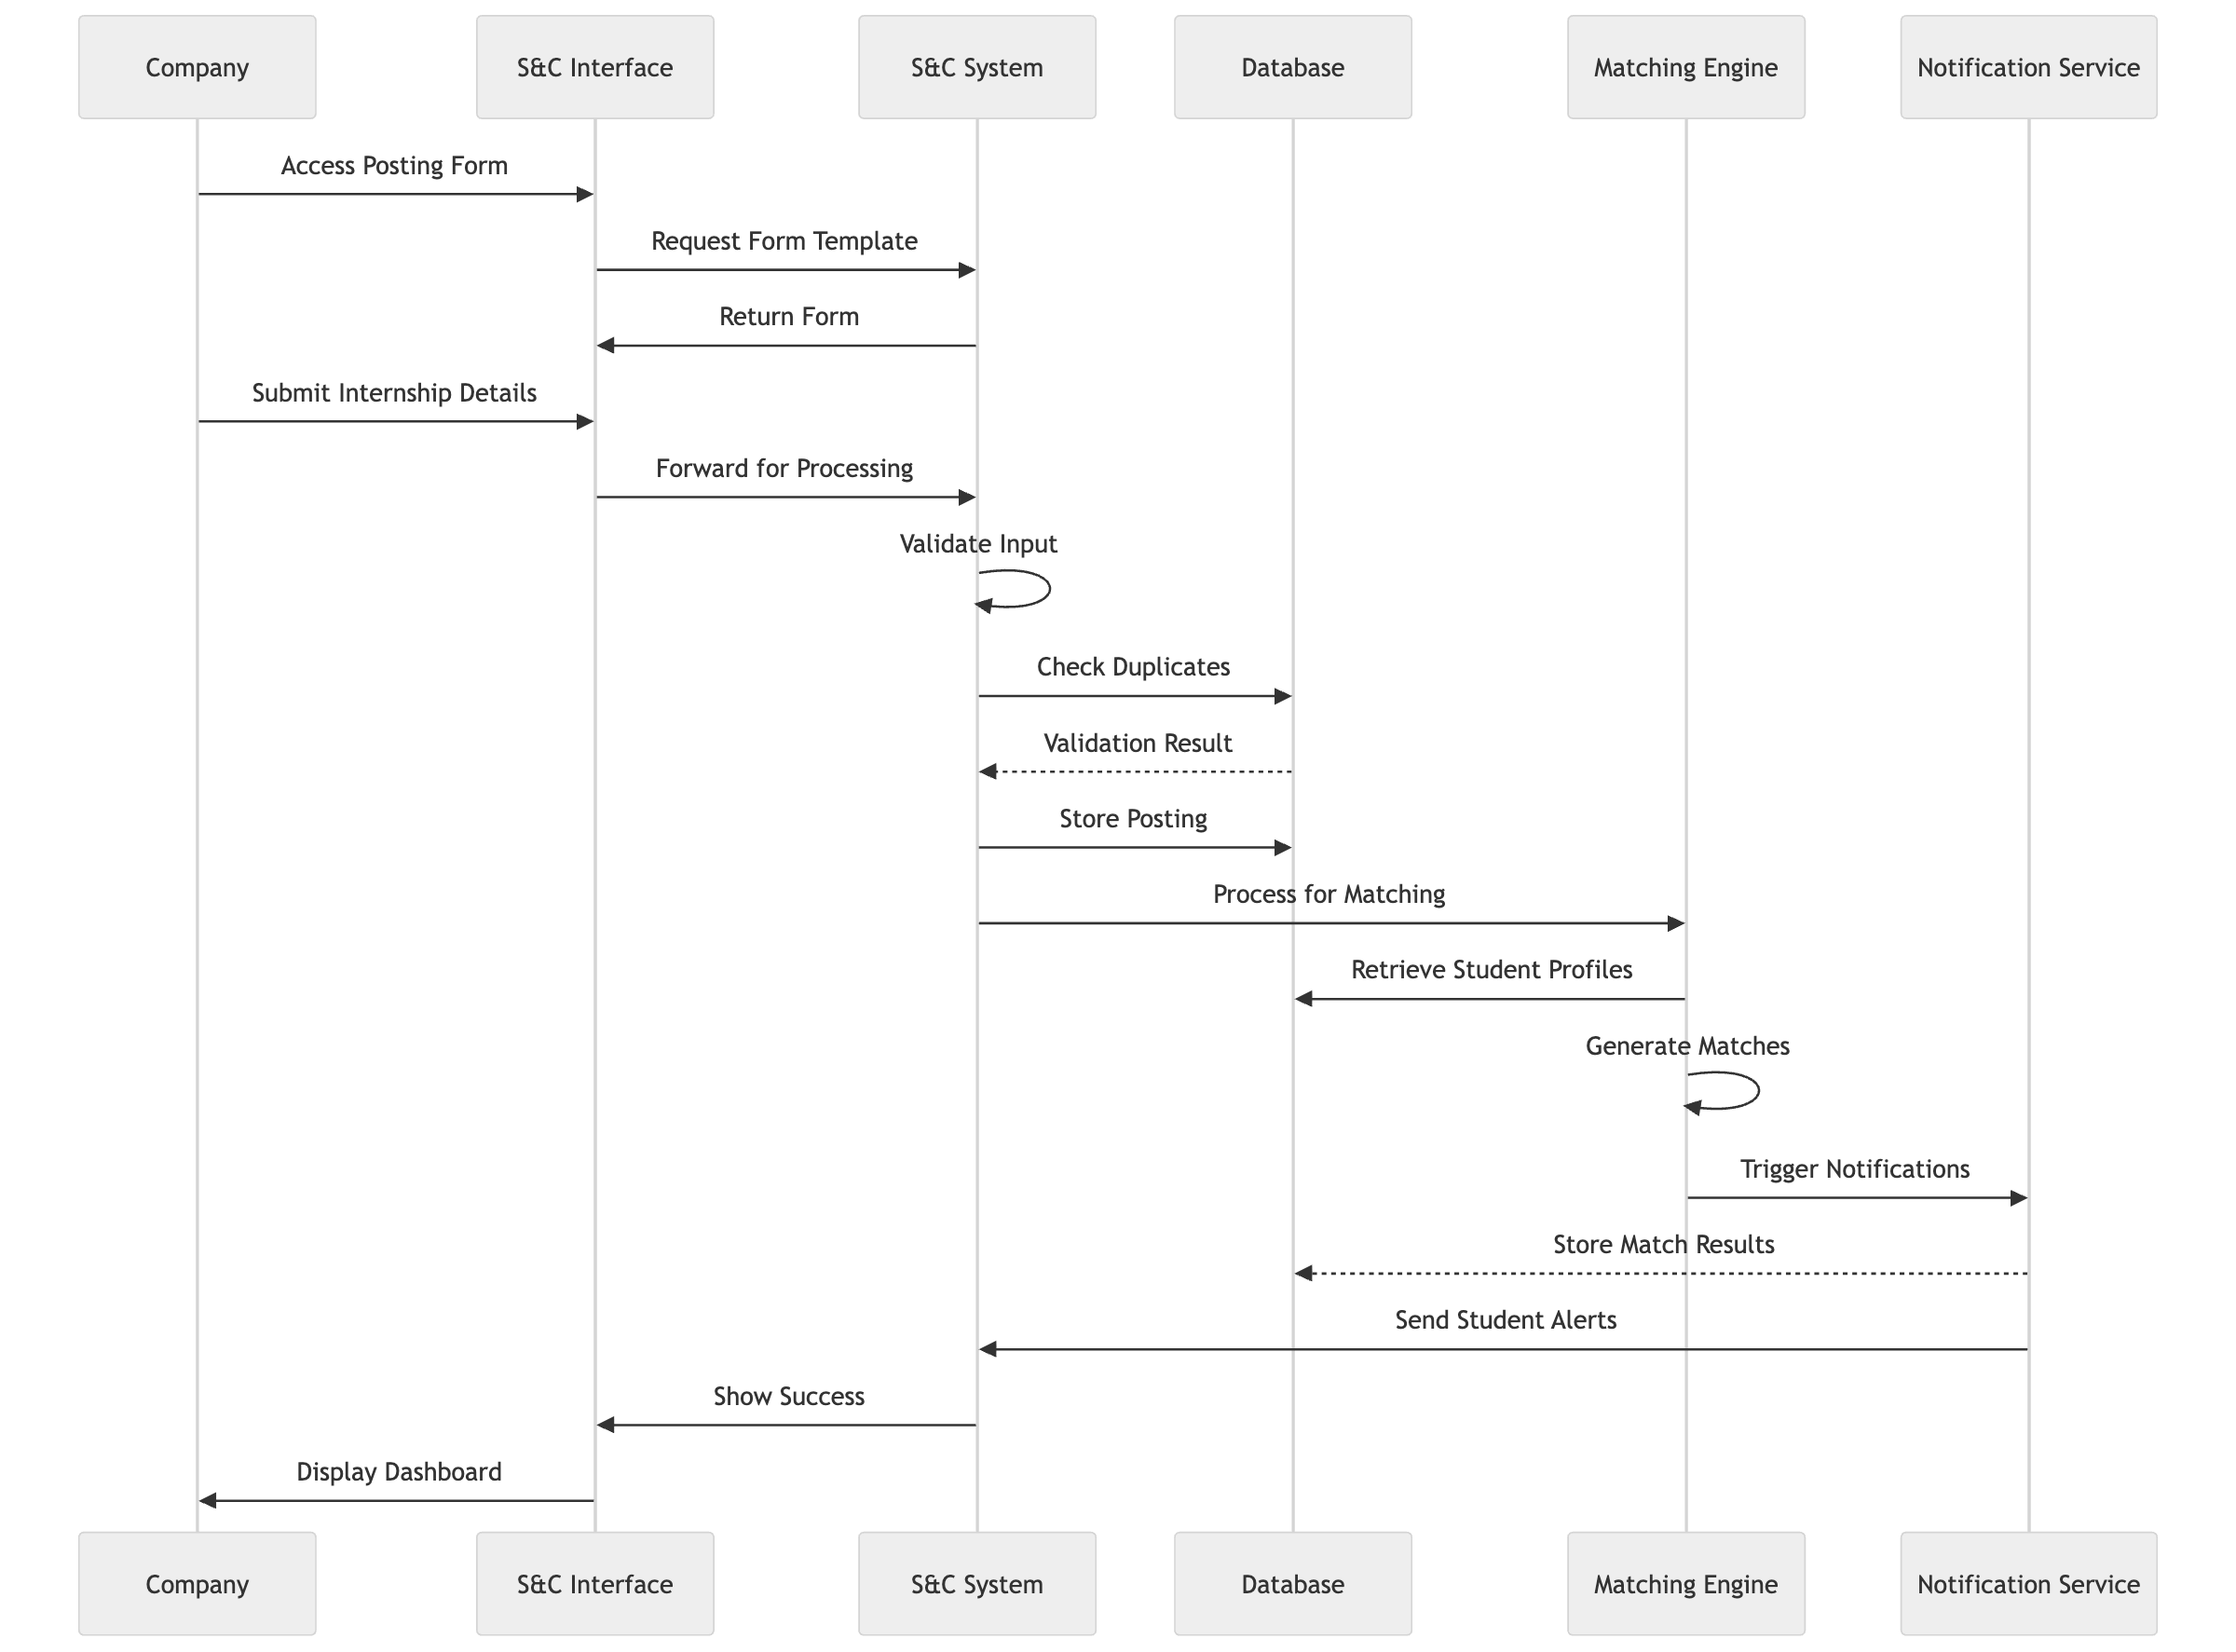
\includegraphics[width=1\linewidth]{JhaBhatiaSharma/Images/Sequence Diagrams/InternshipPosting.png}
        \caption{Sequence Diagram for Internship Posting}
        \label{fig:InternPost}%
    \end{center}
\end{figure}

\subsubsection*{UC\cuc . Student Application Process}
\begin{center}
    \begin{longtable}{|l|p{0.75\linewidth}|}
        \hline
        \textbf{Actor}            & Student \\
        \hline
        \textbf{Entry Conditions} & 
        \begin{itemize}
            \item Student is logged in
            \item Profile and CV are complete
            \item Meets basic internship requirements
        \end{itemize} \\
        \hline
        \textbf{Event Flow}       & 
        \begin{enumerate}
            \item Student finds internship through:
            \begin{itemize}
                \item Direct search
                \item Recommendations
                \item Email notification
            \end{itemize}
            \item Student reviews internship details:
            \begin{itemize}
                \item Company information
                \item Position requirements
                \item Terms and conditions
            \end{itemize}
            \item Student initiates application:
            \begin{itemize}
                \item Selects CV version
                \item Customizes cover letter
                \item Answers screening questions
                \item Provides additional documents
            \end{itemize}
            \item S\&C performs preliminary checks:
            \begin{itemize}
                \item Eligibility verification
                \item Previous applications
                \item Document completeness
            \end{itemize}
            \item Student reviews application package.
            \item Student submits application.
            \item S\&C processes application:
            \begin{itemize}
                \item Updates application counter
                \item Indexes for company search
                \item Generates application ID
            \end{itemize}
            \item Company receives notification.
            \item S\&C updates student dashboard.
            \item Application tracking begins.
        \end{enumerate} \\
        \hline
        \textbf{Exit Conditions}   & 
        \begin{itemize}
            \item Application is submitted
            \item Company is notified
            \item Student can track status
        \end{itemize} \\
        \hline
        \textbf{Exceptions}       & 
        \begin{enumerate}
            \item \textbf{Incomplete Profile:} 
            \begin{itemize}
                \item Redirect to profile completion.
                \item Save application draft.
            \end{itemize} 
            \item \textbf{Missing Required Documents:} \begin{itemize}
                \item List required documents.
                \item Provide upload options.
            \end{itemize} 
            \item \textbf{Previous Application Exists:} \begin{itemize}
                \item Show existing application.
                \item Offer update option.
            \end{itemize} 
            \item \textbf{Deadline Passed:} 
            \begin{itemize}
                \item Show expired notice.
                \item Suggest similar positions.
            \end{itemize} 
            \item \textbf{Requirements Not Met:} 
            \begin{itemize}
                \item Show specific gaps.
                \item Suggest skill development.
            \end{itemize} 
        \end{enumerate} \\
        \hline
        \caption{Student Application Process Use Case.}
        \label{tab:student_application_process_use_case}
    \end{longtable}
\end{center}


\begin{figure}[H]
    \begin{center}
        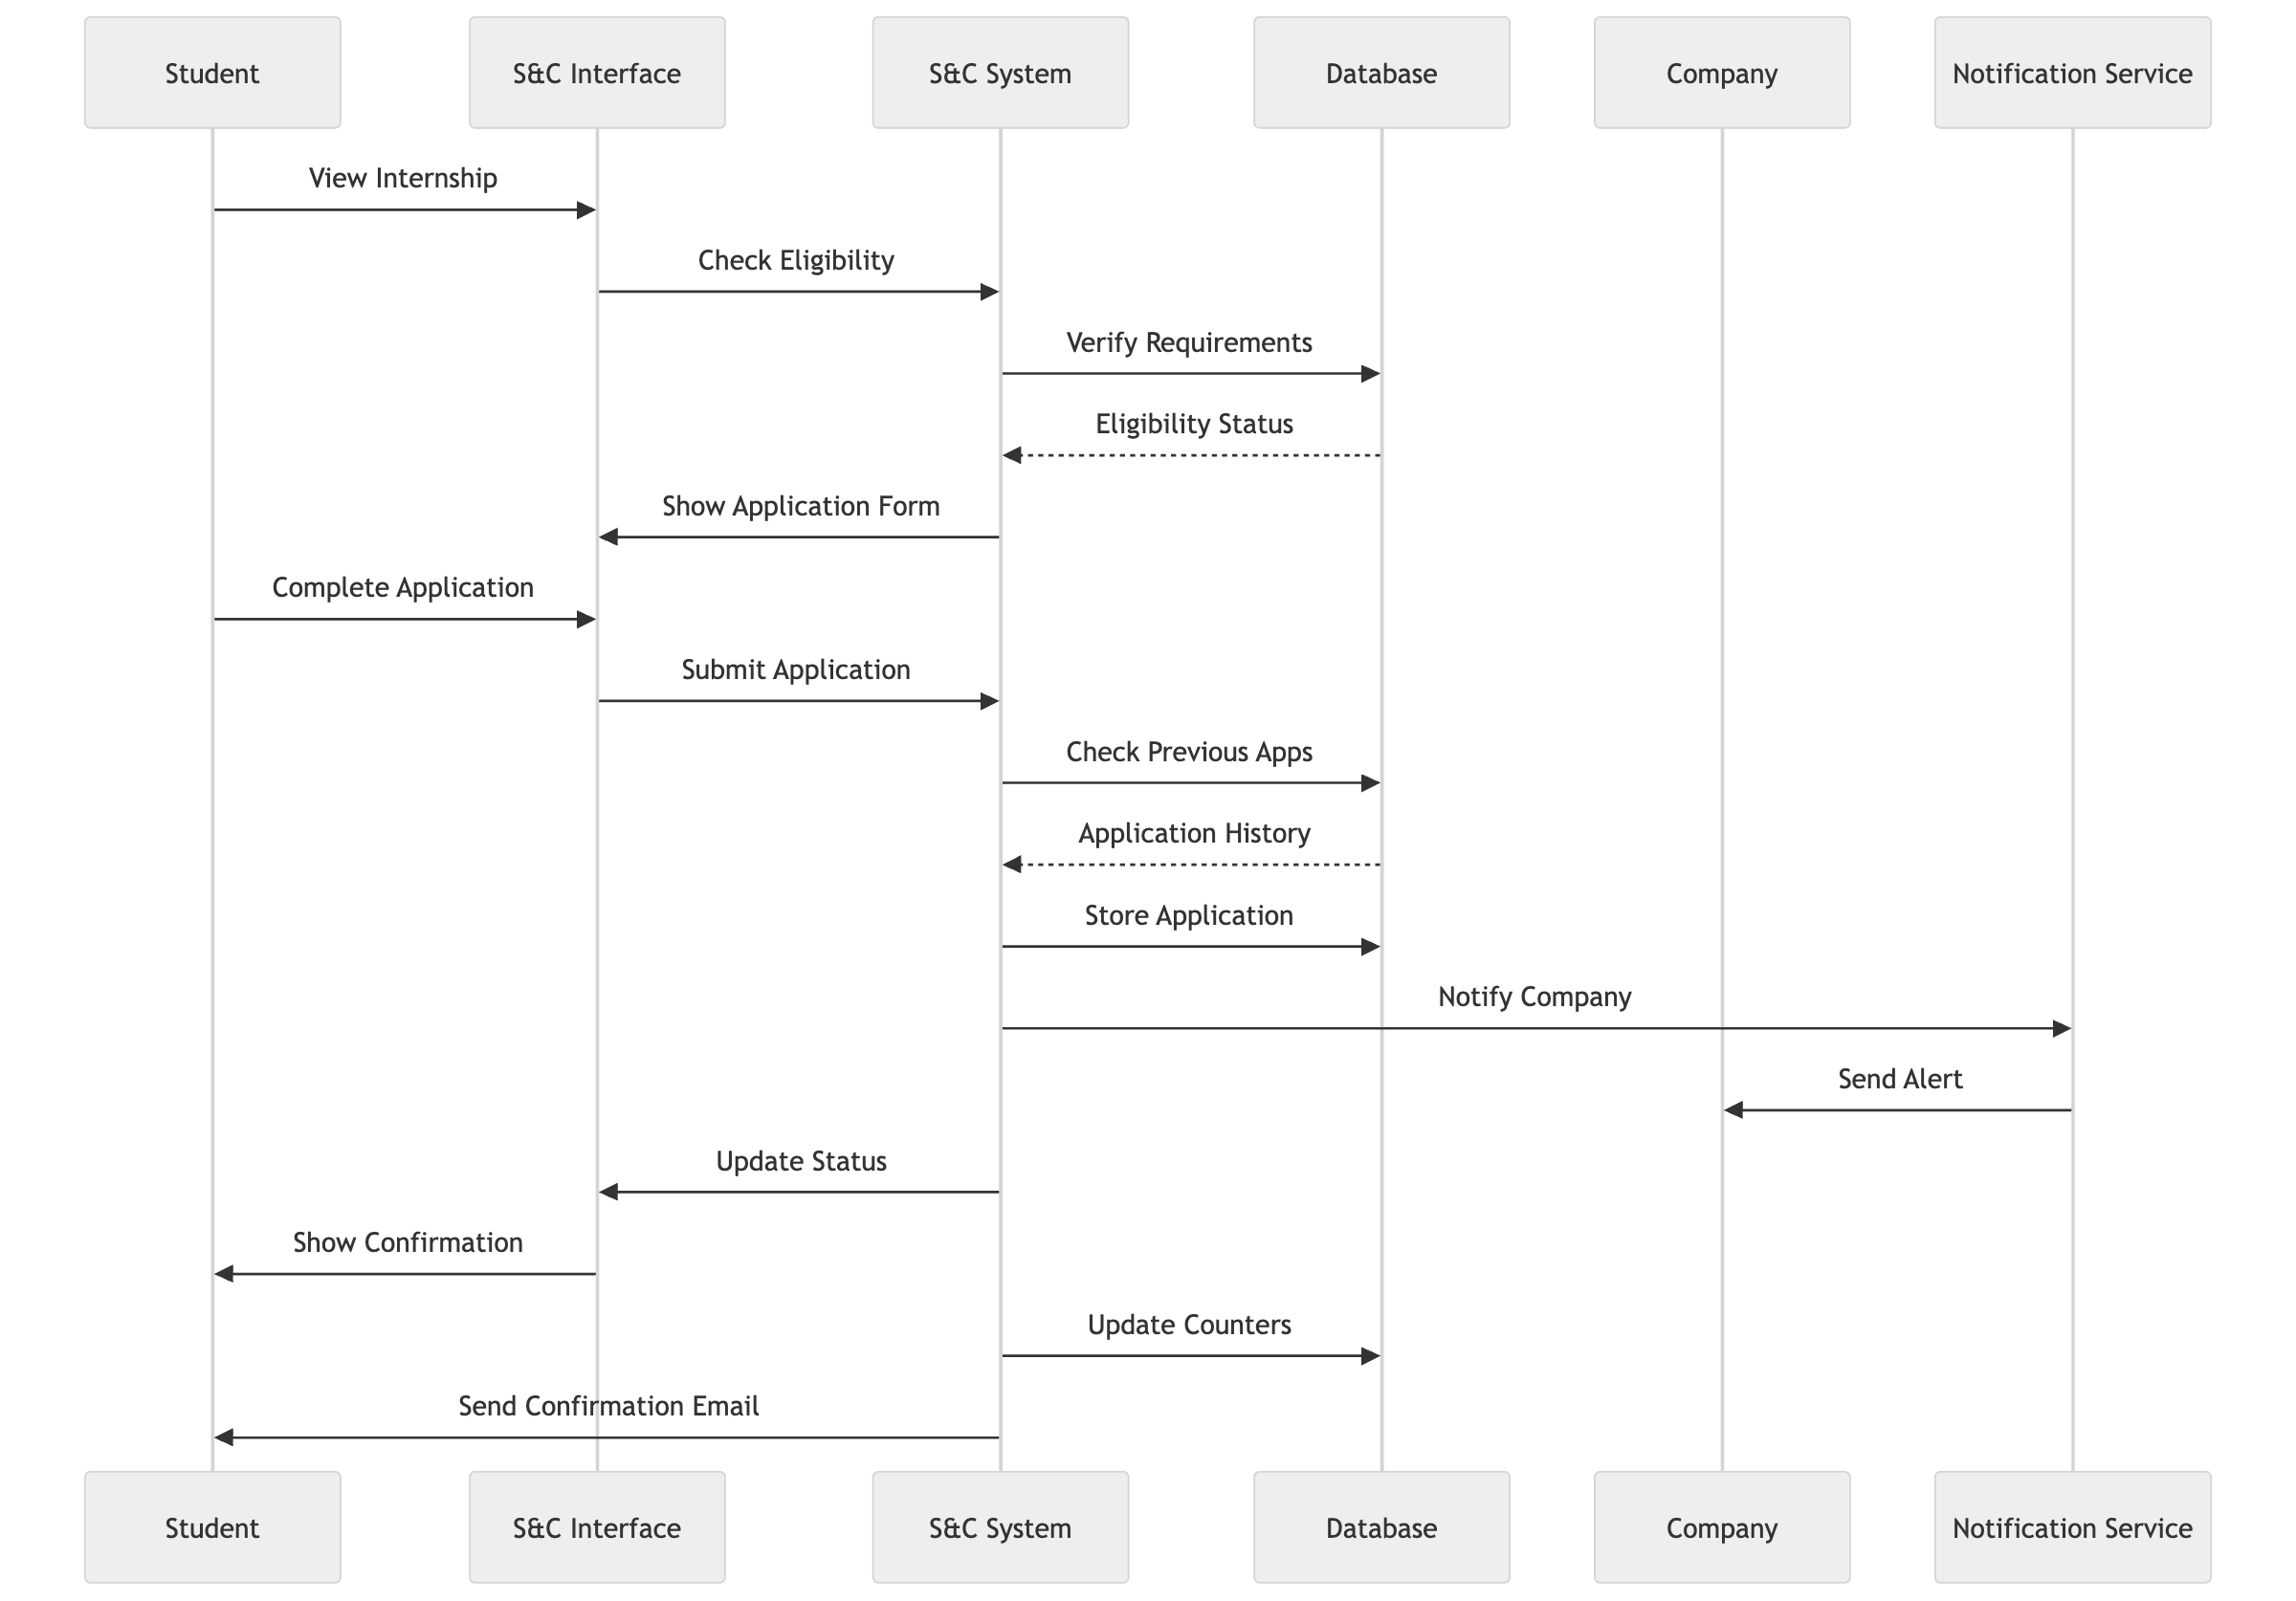
\includegraphics[width=1\linewidth]{JhaBhatiaSharma/Images/Sequence Diagrams/StudentApplication.png}
        \caption{Sequence Diagram for Student Application Process}
        \label{fig:create_a_Tournament_seqd}%
    \end{center}
\end{figure}

\subsubsection*{UC\cuc . Interview Management}
\begin{center}
    \begin{longtable}{|l|p{0.75\linewidth}|}
        \hline
        \textbf{Actor}            & Company Representative, Student \\
        \hline
        \textbf{Entry Conditions} & 
        \begin{itemize}
            \item Application is shortlisted
            \item Both parties are active users
            \item Interview stage is initiated
        \end{itemize} \\
        \hline
        \textbf{Event Flow}       & 
        \begin{enumerate}
            \item Company reviews application.
            \item Company initiates interview process:
            \begin{itemize}
                \item Selects interview type
                \item Proposes time slots
                \item Sets interview format
            \end{itemize}
            \item S\&C sends interview request to student.
            \item Student receives notification:
            \begin{itemize}
                \item Views proposed slots
                \item Checks interview details
                \item Reviews preparations
            \end{itemize}
            \item Student responds:
            \begin{itemize}
                \item Accepts time slot or
                \item Proposes alternatives
            \end{itemize}
            \item S\&C coordinates scheduling:
            \begin{itemize}
                \item Confirms final time
                \item Sends calendar invites
                \item Provides meeting links
            \end{itemize}
            \item Both parties prepare:
            \begin{itemize}
                \item Access interview materials
                \item Review guidelines
                \item Check technical setup
            \end{itemize}
            \item Interview conducted.
            \item Company provides feedback:
            \begin{itemize}
                \item Evaluation form
                \item Notes and ratings
                \item Decision input
            \end{itemize}
            \item S\&C processes results:
            \begin{itemize}
                \item Updates application status
                \item Notifies student
                \item Records outcomes
            \end{itemize}
        \end{enumerate} \\
        \hline
        \textbf{Exit Conditions}   & 
        \begin{itemize}
            \item Interview is completed
            \item Feedback is recorded
            \item Next steps are initiated
        \end{itemize} \\
        \hline
        \textbf{Exceptions}       & 
        \begin{enumerate}
            \item \textbf{Schedule Conflicts:}
            \begin{itemize}
                \item Rescheduling process
                \item Alternative slot suggestions
            \end{itemize}
            \item \textbf{Technical Issues:}
            \begin{itemize}
                \item Backup contact methods
                \item Rescheduling options
            \end{itemize}
            \item \textbf{No-Show Scenarios:}
            \begin{itemize}
                \item Record incident
                \item Reschedule policy
            \end{itemize}
            \item \textbf{Cancellation Requests:}
            \begin{itemize}
                \item Process cancellation
                \item Update status
            \end{itemize}
            \item \textbf{Feedback Deadline Missed:}
            \begin{itemize}
                \item Send reminders
                \item Escalation process
            \end{itemize}
        \end{enumerate} \\
        \hline
        \caption{Interview Management Use Case.}
        \label{tab:interview_management_use_case}
    \end{longtable}
\end{center}


\begin{figure}[H]
    \begin{center}
        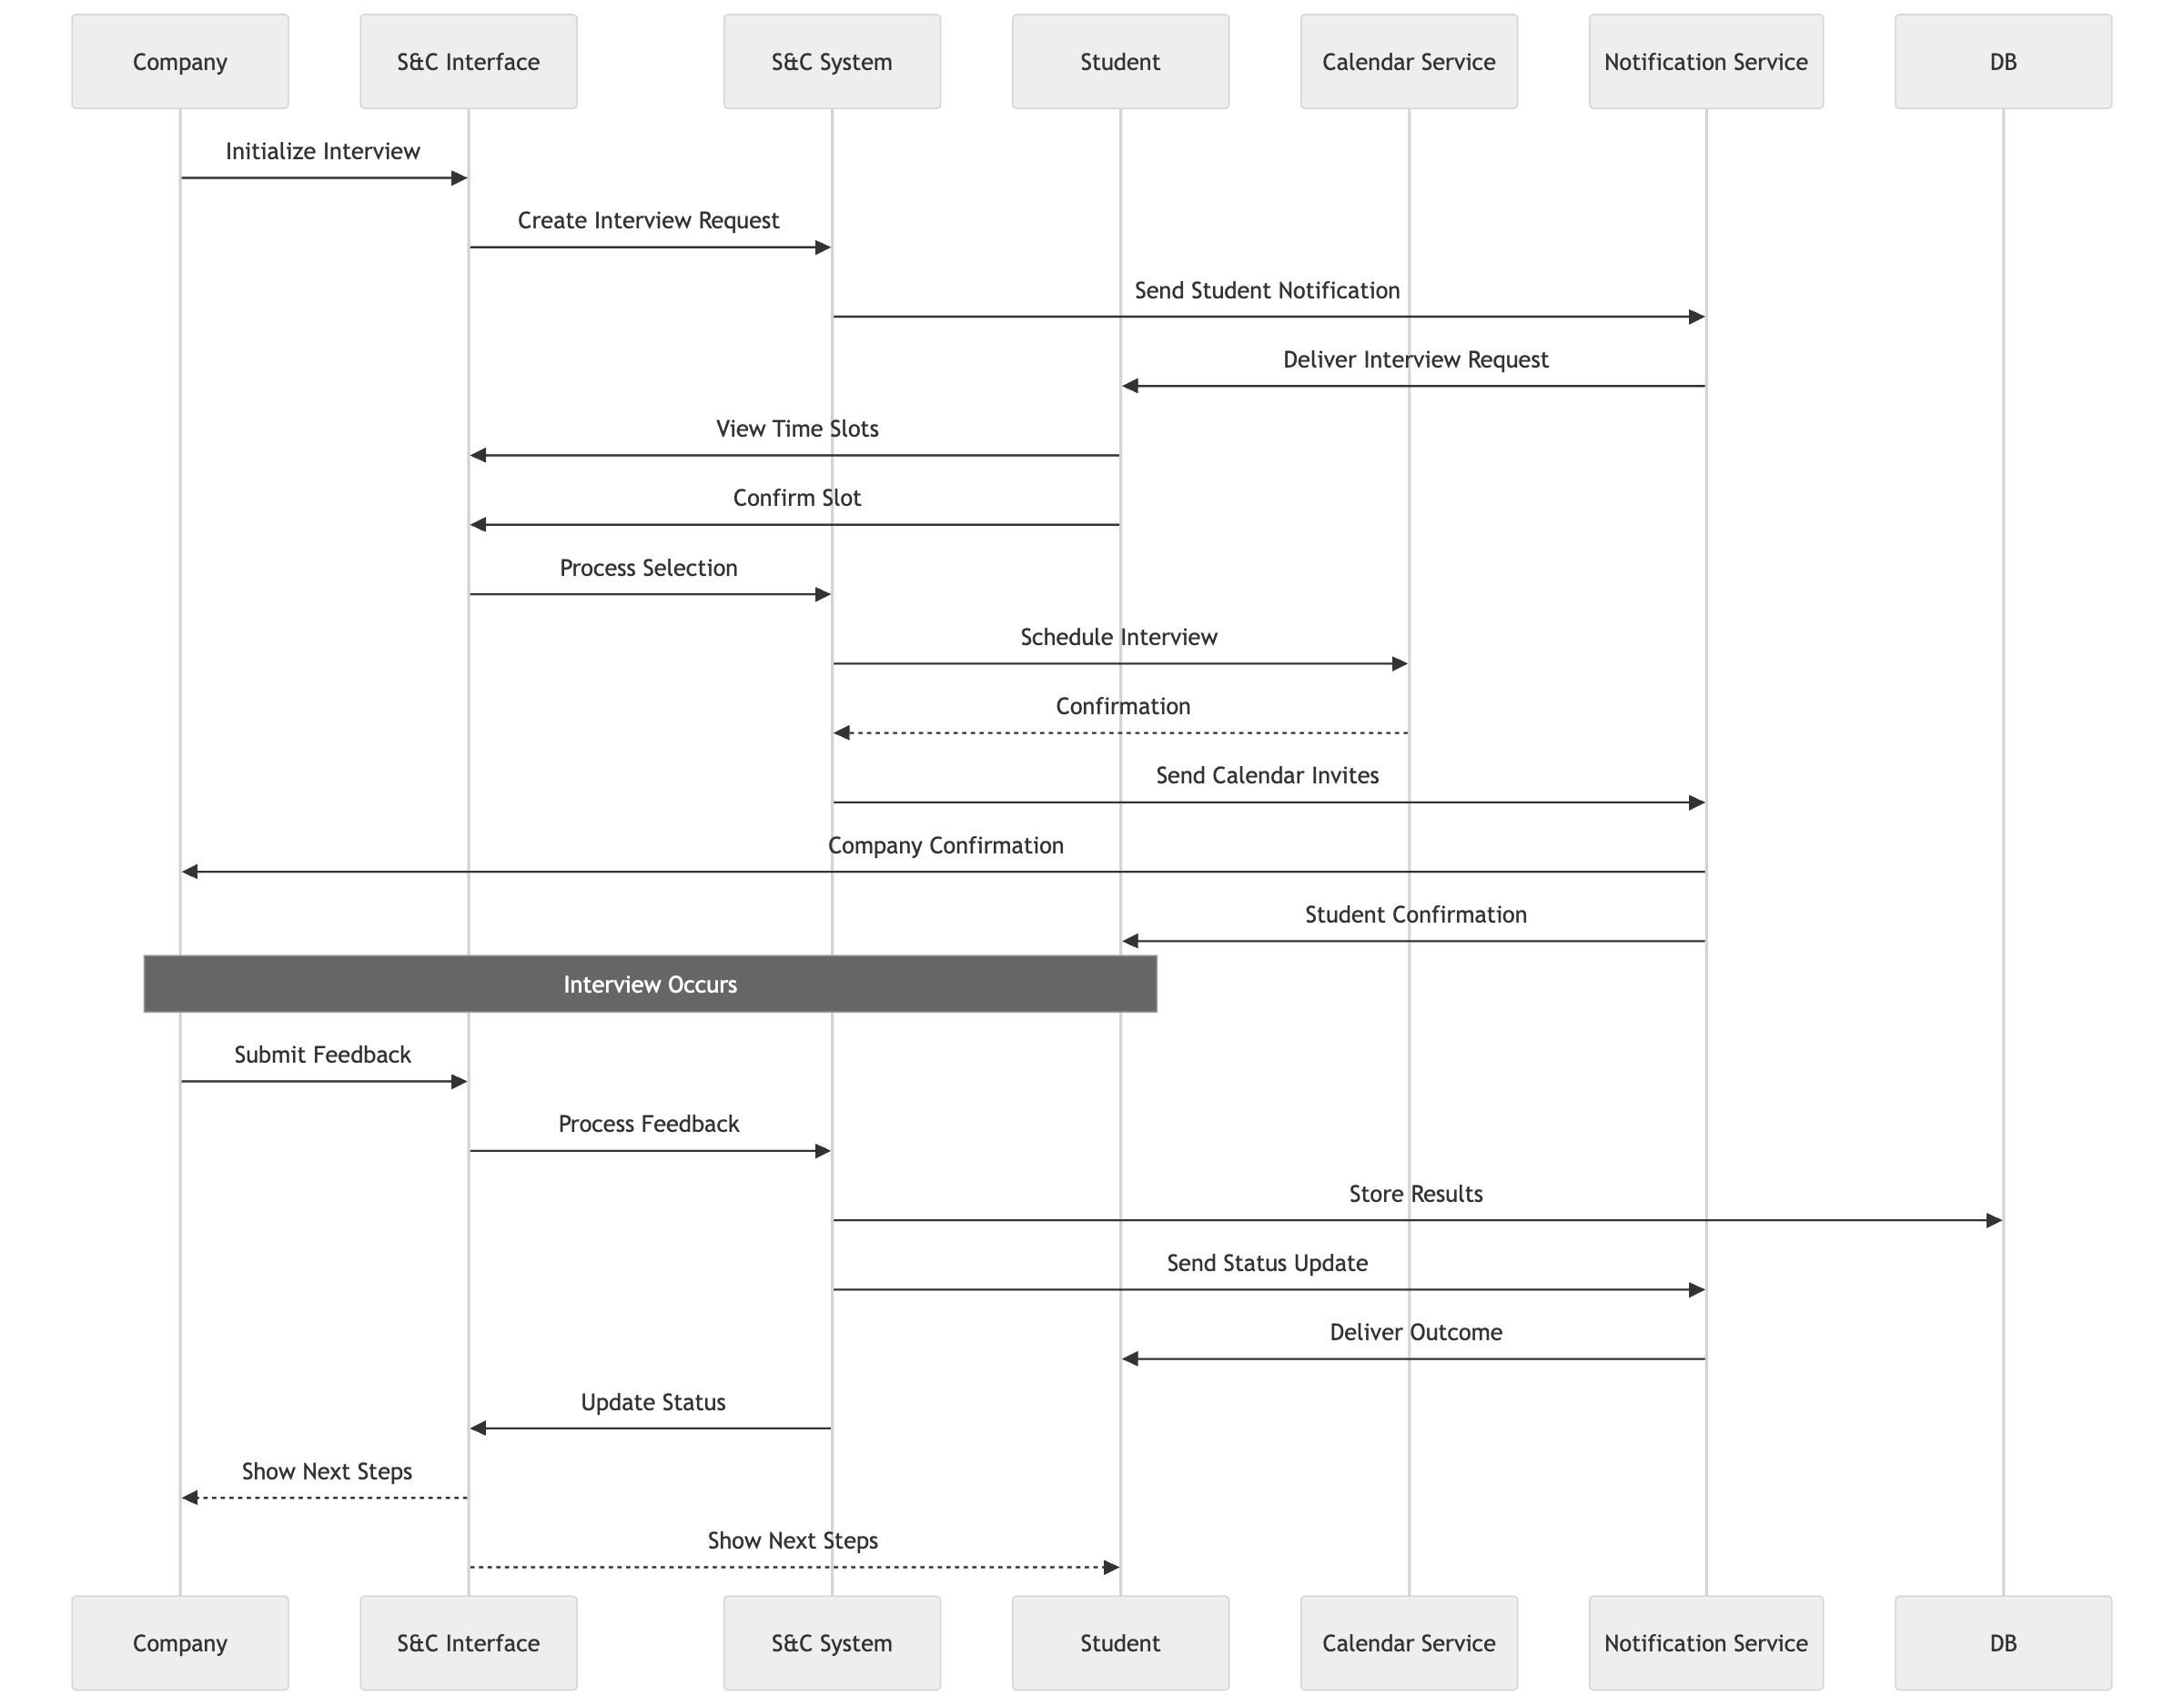
\includegraphics[width=1\linewidth]{JhaBhatiaSharma/Images/Sequence Diagrams/InterviewManagement.png}
        \caption{Sequence Diagram for Interview Management}
        \label{fig:join_a_Tournament_seqd}%
    \end{center}
\end{figure}

\subsubsection*{UC\cuc . Complaint Handling}
\begin{center}
    \begin{longtable}{|l|p{0.75\linewidth}|}
        \hline
        \textbf{Actor}            & Student/Company, University Administrator \\
        \hline
        \textbf{Entry Conditions} & 
        \begin{itemize}
            \item User is registered and active
            \item Incident is within platform scope
            \item Related internship is active/recent
        \end{itemize} \\
        \hline
        \textbf{Event Flow}       & 
        \begin{enumerate}
            \item User initiates complaint:
            \begin{itemize}
                \item Selects complaint type
                \item Identifies involved parties
                \item Describes incident
                \item Provides evidence
            \end{itemize}
            \item S\&C processes submission:
            \begin{itemize}
                \item Assigns complaint ID
                \item Categorizes severity
                \item Routes to appropriate admin
            \end{itemize}
            \item Administrator receives case:
            \begin{itemize}
                \item Reviews details
                \item Assesses priority
                \item Initiates investigation
            \end{itemize}
            \item S\&C facilitates investigation:
            \begin{itemize}
                \item Gathers additional information
                \item Contacts involved parties
                \item Documents communications
            \end{itemize}
            \item Administrator actions:
            \begin{itemize}
                \item Reviews all evidence
                \item Consults policies
                \item Determines resolution
            \end{itemize}
            \item Resolution implementation:
            \begin{itemize}
                \item Notifies all parties
                \item Records decisions
                \item Implements actions
            \end{itemize}
            \item Follow-up process:
            \begin{itemize}
                \item Monitors compliance
                \item Collects feedback
                \item Updates records
            \end{itemize}
        \end{enumerate} \\
        \hline
        \textbf{Exit Conditions}   & 
        \begin{itemize}
            \item Complaint is resolved
            \item Actions are implemented
            \item Resolution is documented
        \end{itemize} \\
        \hline
        \textbf{Exceptions}       & 
        \begin{enumerate}
            \item \textbf{Insufficient Information:} 
            \begin{itemize}
                \item Request additional details.
                \item Hold complaint status.
            \end{itemize} 
            \item \textbf{Multiple Parties Involved:} 
            \begin{itemize}
                \item Expand investigation scope.
                \item Coordinate responses.
            \end{itemize} 
            \item \textbf{Policy Violations Found:}
            \begin{itemize}
                \item Escalate to higher authority.
                \item Implement immediate actions.
            \end{itemize} 
            \item \textbf{Appeal Submitted:} 
            \begin{itemize}
                \item Review appeal grounds.
                \item Reassign to different admin.
            \end{itemize} 
            \item \textbf{Resolution Deadline Missed:} 
            \begin{itemize}
                \item Escalate to supervisor.
                \item  Update timeline.
            \end{itemize}
        \end{enumerate} \\
        \hline
        \caption{Complaint Handling Use Case.}
        \label{tab:complaint_handling_use_case}
    \end{longtable}
\end{center}


\begin{figure}[H]
    \begin{center}
        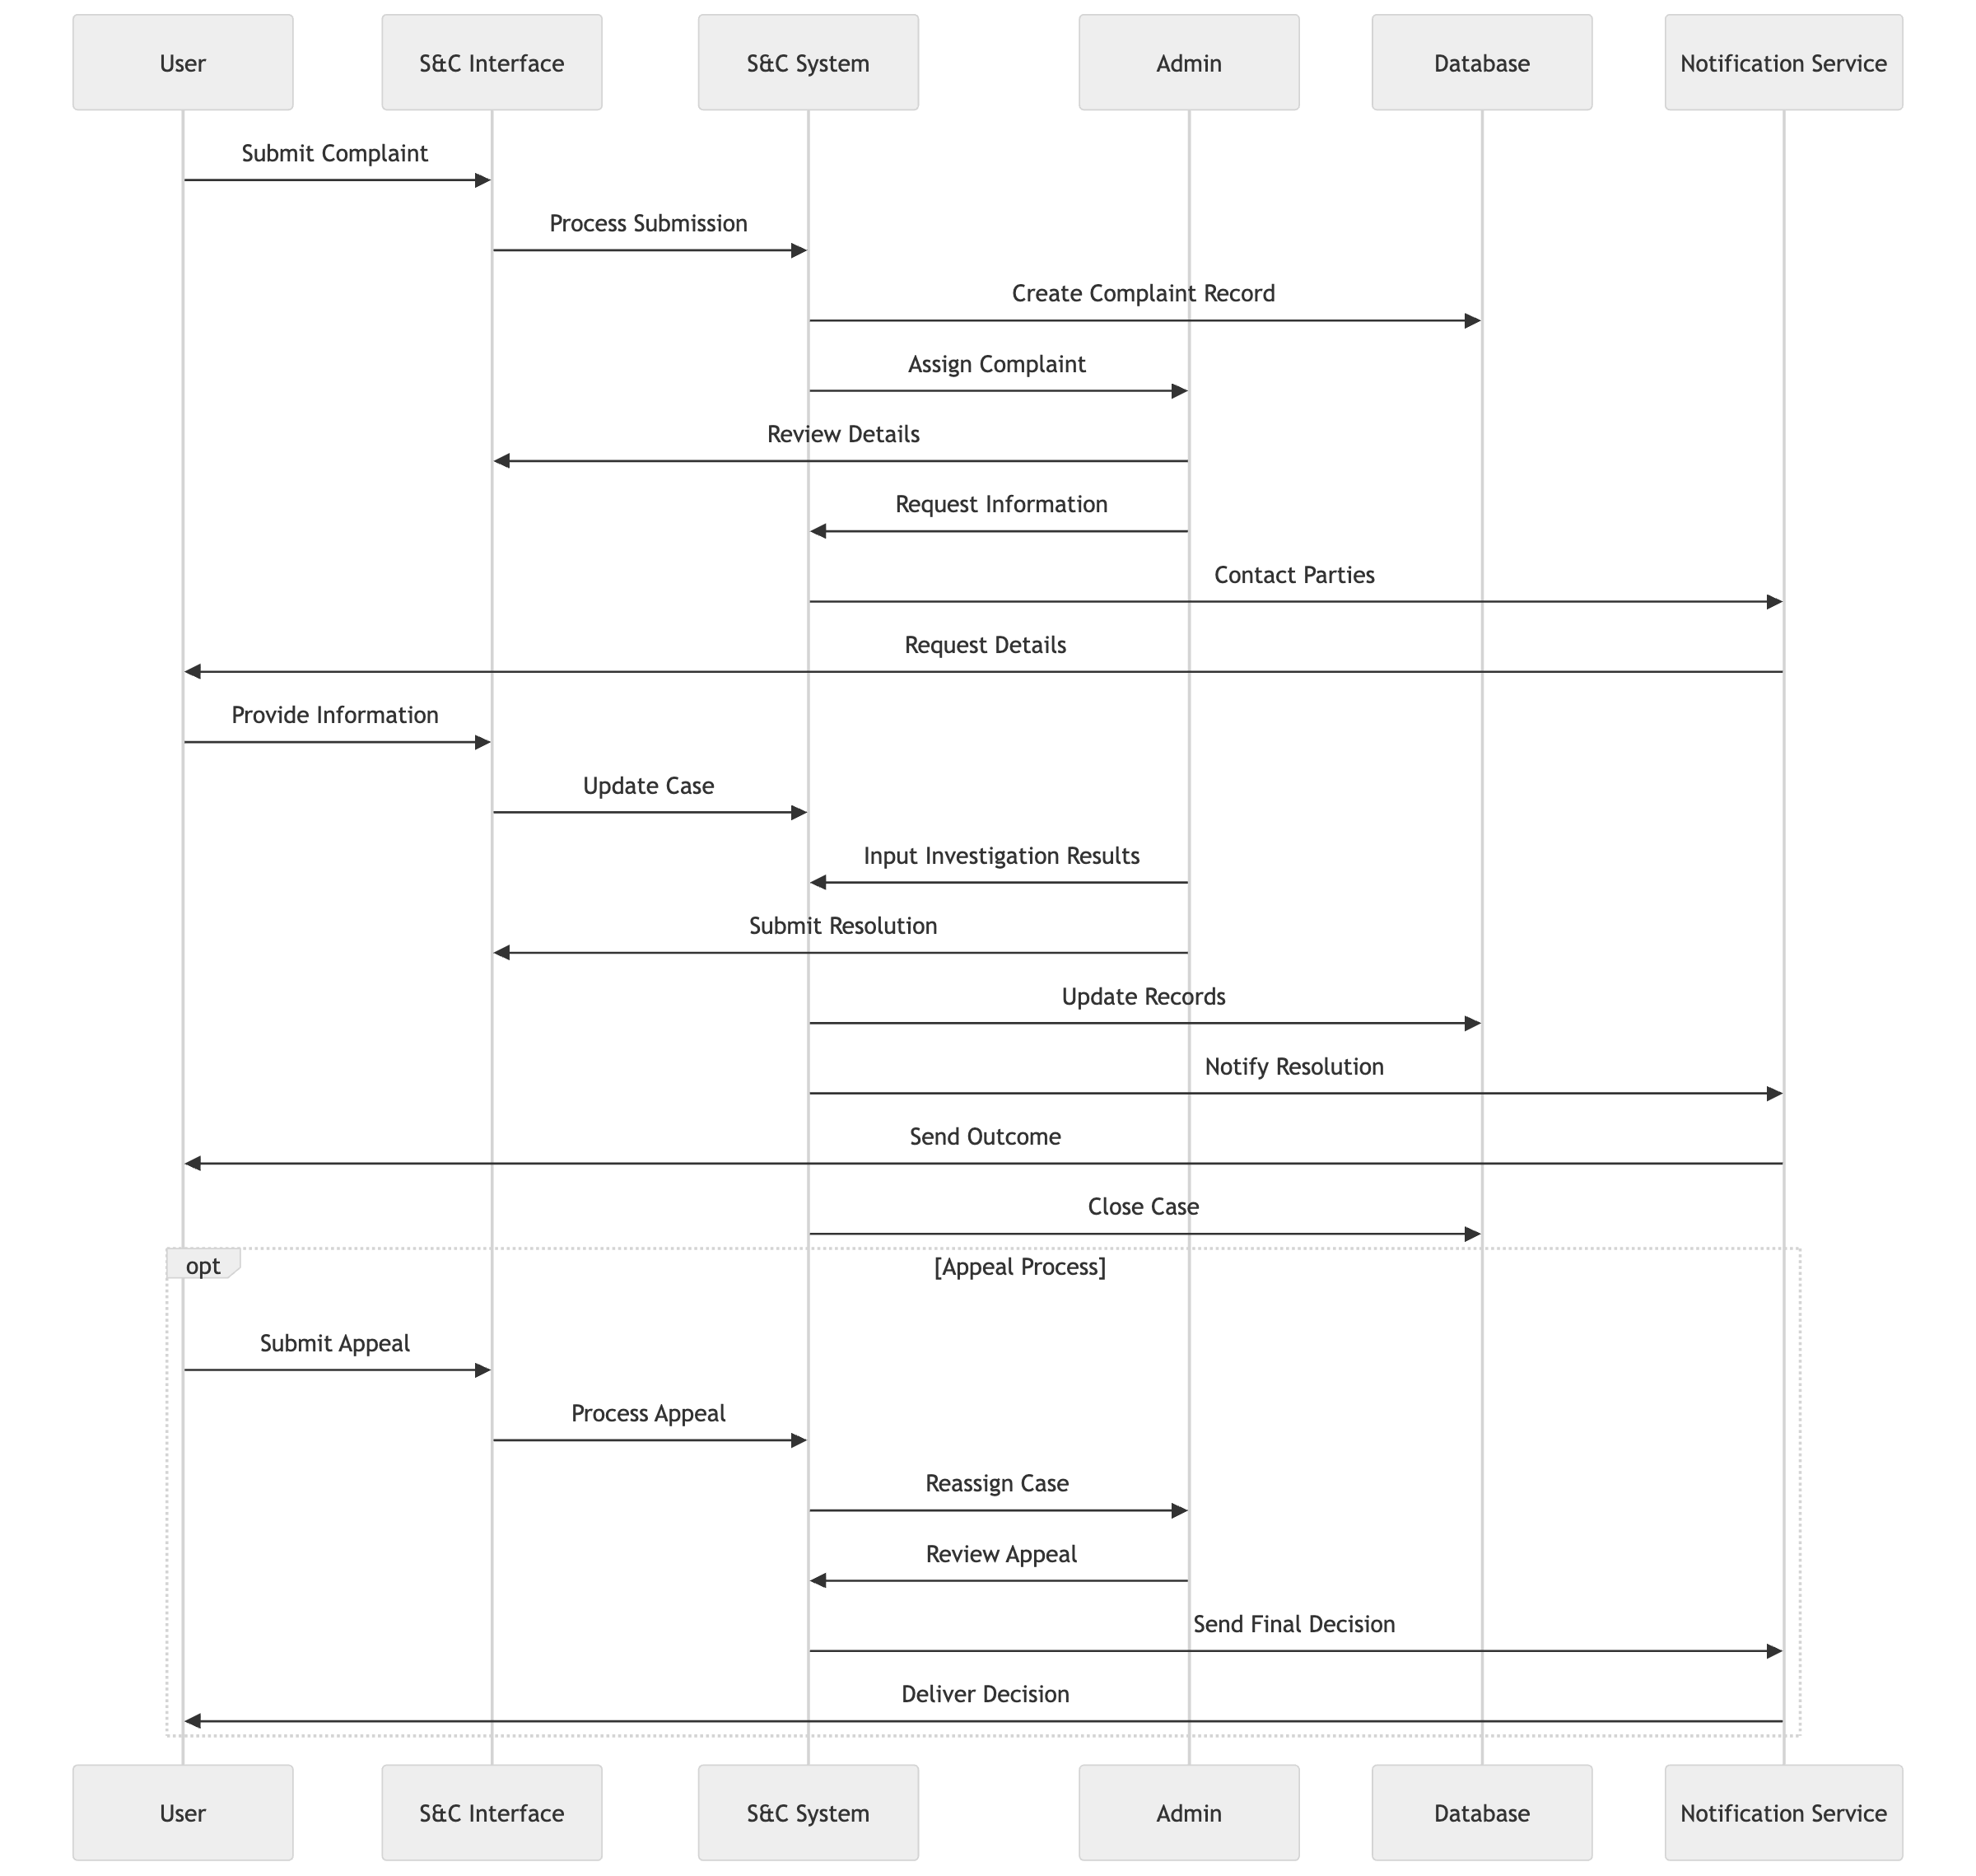
\includegraphics[width=1\linewidth]{JhaBhatiaSharma/Images/Sequence Diagrams/ComplaintHandling.png}
        \caption{Sequence Diagram for Complaint Handling}
        \label{fig:ComplainHandling}%
    \end{center}
\end{figure}

\subsubsection*{UC\cuc . Admin Privileges}
\begin{longtable}{|l|p{0.75\linewidth}|}
    \hline
    \textbf{Actor}            & University Administrator \\
    \hline
    \textbf{Entry Conditions} & 
    \begin{itemize}
        \item Admin is logged in with verification privileges
        \item Items pending verification exist
        \item Access to verification tools available
    \end{itemize} \\
    \hline
    \textbf{Event Flow}       & 
    \begin{enumerate}
        \item Admin accesses verification dashboard:
        \begin{itemize}
            \item Views pending items
            \item Checks verification queue
            \item Reviews priority items
        \end{itemize}
        \item For each verification request:
        \begin{itemize}
            \item Reviews company details
            \item Checks documentation
            \item Validates credentials
            \item Assesses compliance
        \end{itemize}
        \item Document verification:
        \begin{itemize}
            \item Company registration
            \item Business licenses
            \item Insurance certificates
            \item Tax documentation
        \end{itemize}
        \item Compliance check:
        \begin{itemize}
            \item University policies
            \item Legal requirements
            \item Industry standards
            \item Safety regulations
        \end{itemize}
        \item Decision process:
        \begin{itemize}
            \item Approves application
            \item Requests modifications
            \item Rejects with reason
        \end{itemize}
        \item Post-approval actions:
        \begin{itemize}
            \item Sets verification status
            \item Assigns trust score
            \item Enables features
            \item Sets review date
        \end{itemize}
        \item Communication:
        \begin{itemize}
            \item Notifies company
            \item Updates records
            \item Documents decision
        \end{itemize}
    \end{enumerate} \\
    \hline
    \textbf{Exit Conditions}   & 
    \begin{itemize}
        \item Verification decision made
        \item Company notified
        \item Records updated
    \end{itemize} \\
    \hline
    \textbf{Exceptions}       & 
    \begin{enumerate}
        \item \textbf{Missing Documentation:}
        \begin{itemize}
            \item Request specific documents
            \item Set pending status
        \end{itemize}
        \item \textbf{Compliance Issues:}
        \begin{itemize}
            \item Detail requirements
            \item Provide guidance
        \end{itemize}
        \item \textbf{Verification Timeout:}
        \begin{itemize}
            \item Extend deadline
            \item Notify parties
        \end{itemize}
        \item \textbf{Suspicious Activity:}
        \begin{itemize}
            \item Flag for investigation
            \item Suspend processing
        \end{itemize}
        \item \textbf{Appeal Request:}
        \begin{itemize}
            \item Review appeal
            \item Escalate if needed
        \end{itemize}
    \end{enumerate} \\
    \hline
    \caption{Admin Privileges Use Case.}
    \label{tab:admin_privileges_use_case}
\end{longtable}

\begin{figure}[H]
    \begin{center}
        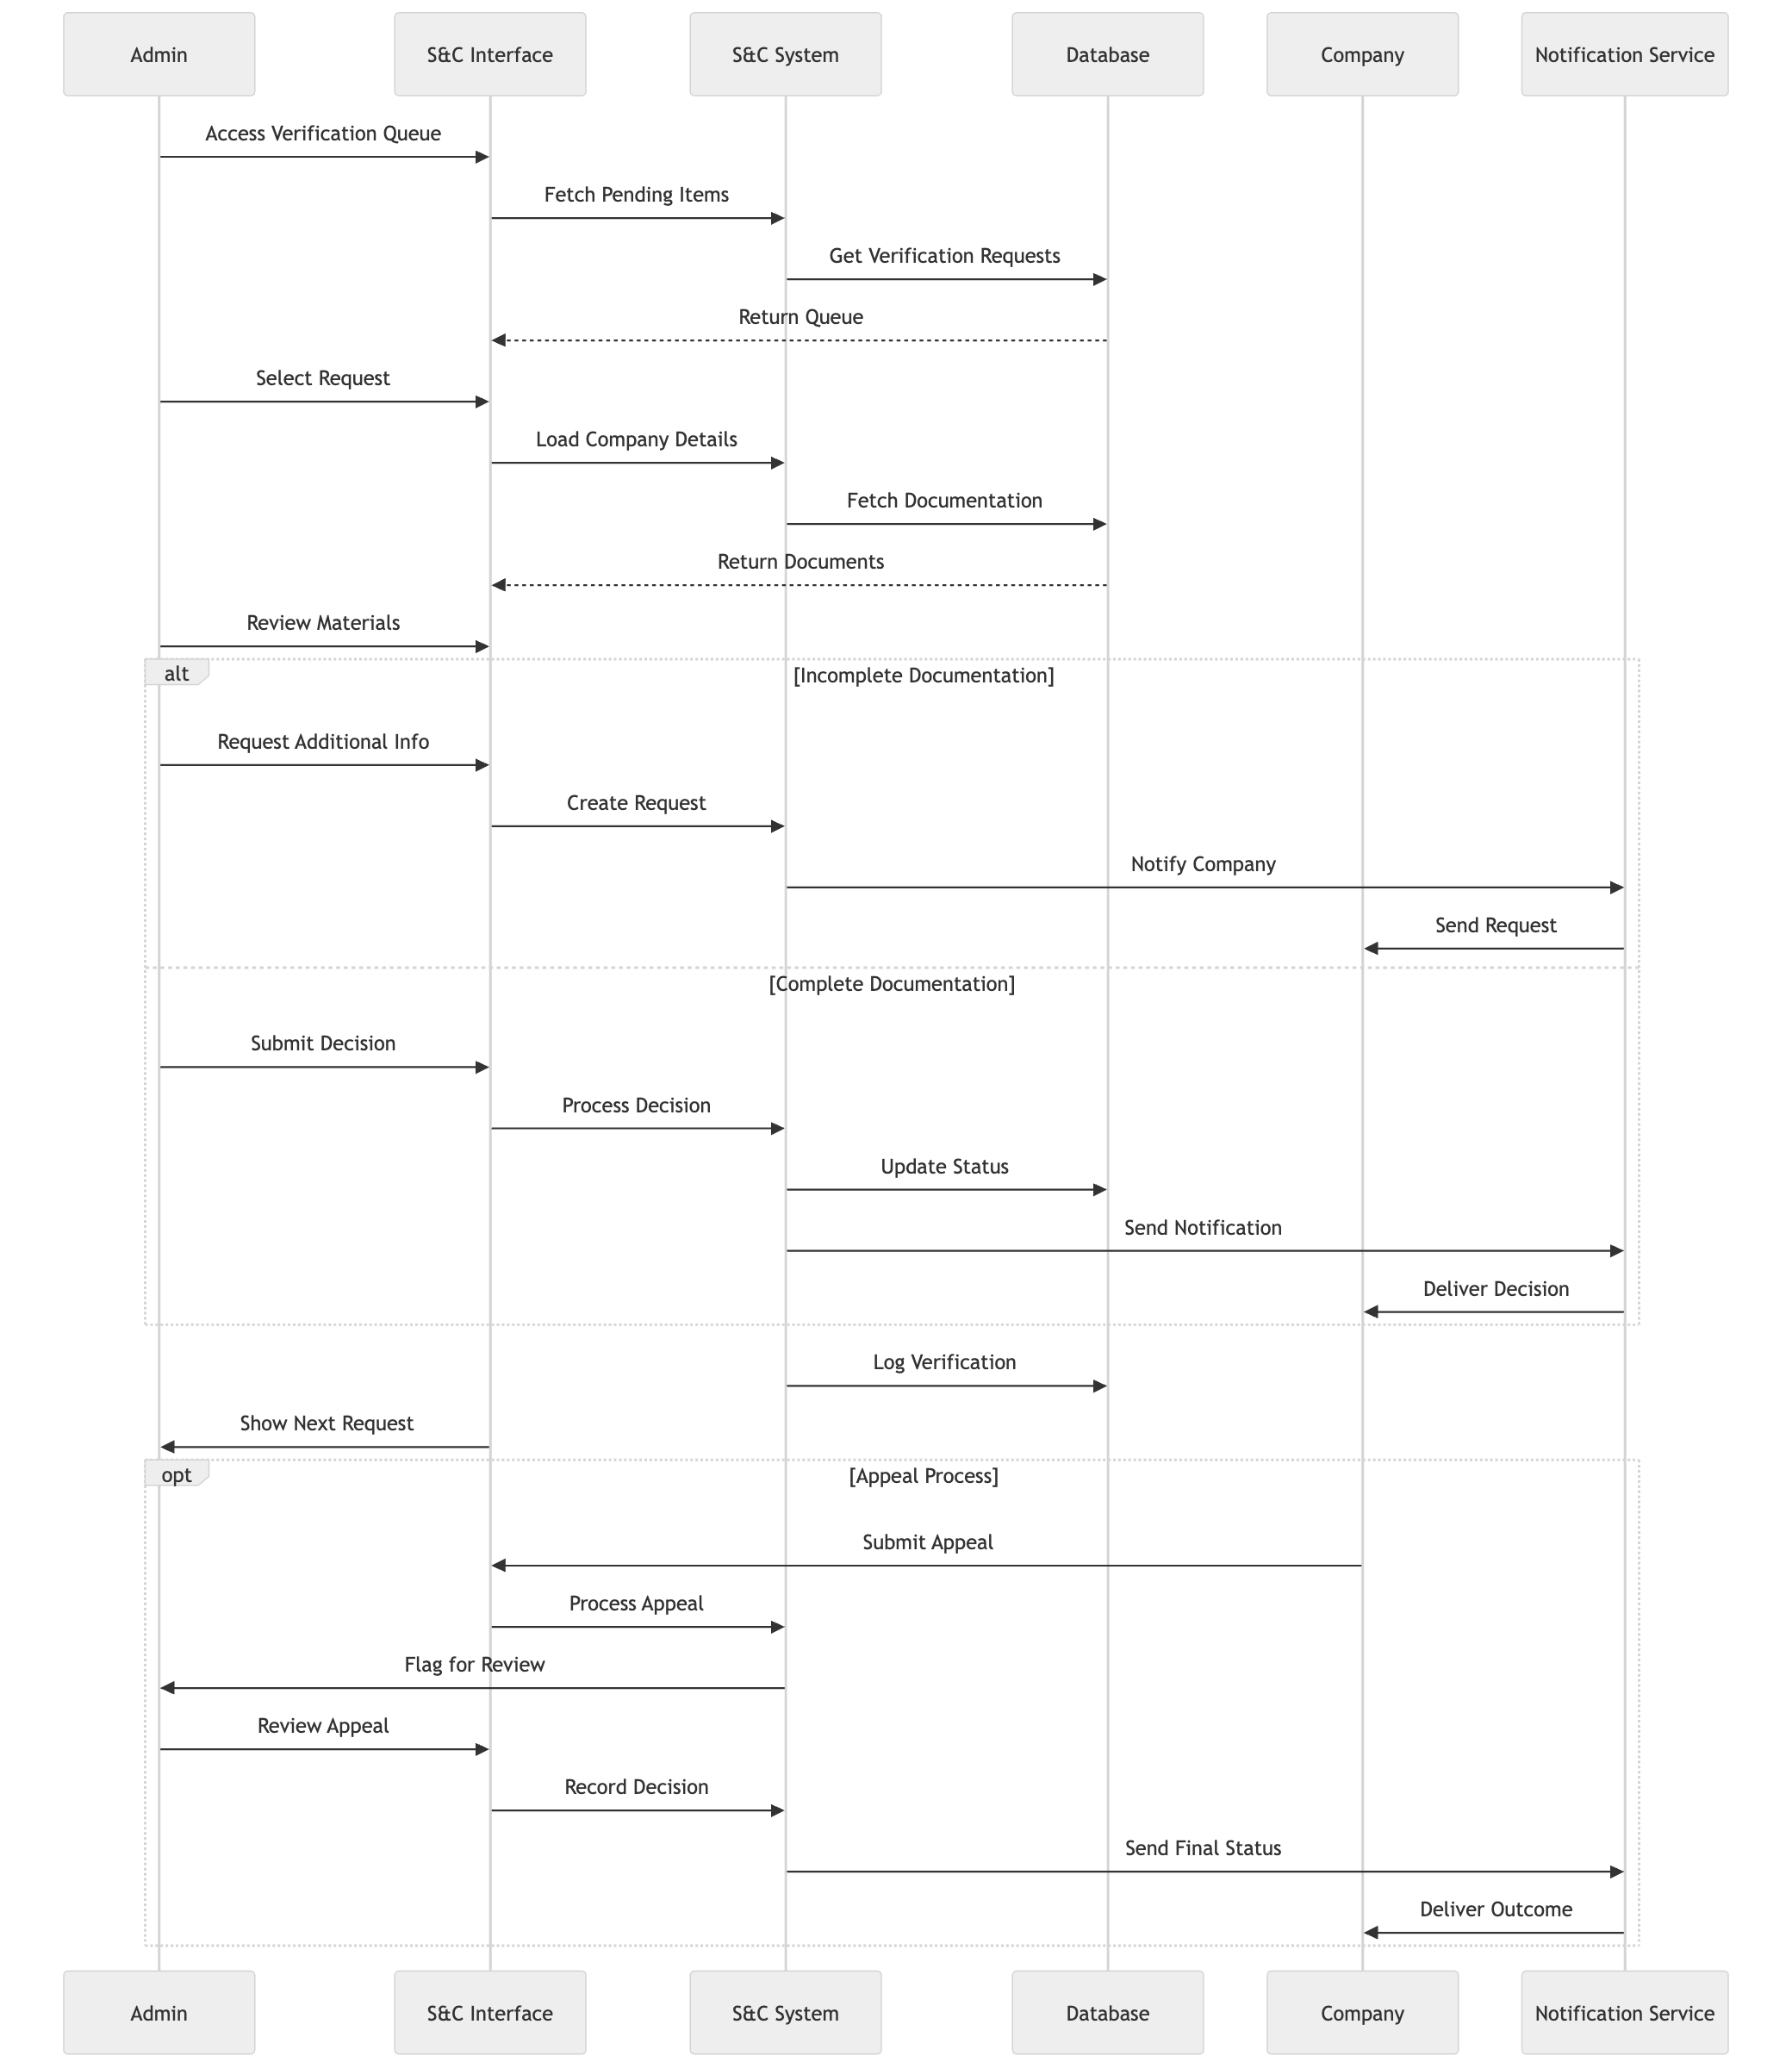
\includegraphics[width=1\linewidth]{JhaBhatiaSharma/Images/Sequence Diagrams/AdminPriviliges.png}
        \caption{Sequence Diagram for Admin Privileges}
        \label{fig:adminPrivileges}%
    \end{center}
\end{figure}
\newpage

\subsection{Performance Requirements}
\label{subsec:performance_requirements}

\subsubsection*{Response Time}
\begin{itemize}
    \item \textbf{Page Load:} Less than \textbf{5 seconds} for typical pages during testing.
    \item \textbf{Search Results:} Less than \textbf{2 seconds} for small-scale datasets.
    \item \textbf{File Upload:} Less than \textbf{10 seconds} for files up to \textbf{10MB}.
    \item \textbf{Real-time Updates:} Less than \textbf{1 second} for key interactive features.
\end{itemize}

\subsubsection*{System Capacity}
\begin{itemize}
    \item \textbf{Concurrent Users:} Support for up to \textbf{50 simultaneous users}.
    \item \textbf{Database Transactions:} Designed to handle \textbf{10 transactions per second} under typical usage.
    \item \textbf{File Storage:} Capacity for up to \textbf{10GB}, suitable for project scope and testing.
    \item \textbf{Backup Frequency:} \textbf{Weekly or manual backups} for data protection during development.
\end{itemize}

\subsubsection*{Availability}
\begin{itemize}
    \item \textbf{Uptime:} \textbf{Target of 95\%}, considering potential downtime for development and testing.
    \item \textbf{Scheduled Maintenance:} As needed during the project lifecycle.
    \item \textbf{Backup Recovery:} Recovery within \textbf{12 hours for small-scale data}.
    \item \textbf{Error Rate:} Less than \textbf{1\% for prototype-level functionality}.
\end{itemize}


\newpage
\section{Design constraints}
\label{sec:design_constraints}%


\subsection{Design Constraints}
\label{subsec:design_constraints}

\subsubsection*{Standards Compliance}
\begin{itemize}
    \item \textbf{GDPR Compliance:} 
    The platform must comply with the \textbf{General Data Protection Regulation} to ensure the protection of user data and privacy. This includes explicit consent mechanisms, data anonymization, and secure data processing protocols.
    \item \textbf{WCAG 2.1 Accessibility:} 
    Adheres to the \textbf{Web Content Accessibility Guidelines 2.1} to ensure inclusivity. This involves providing support for screen readers, keyboard navigation, and ensuring sufficient color contrast.
    \item \textbf{ISO/IEC 27001 Security:} 
    Implements security management practices aligned with \textbf{ISO/IEC 27001} to safeguard information assets and prevent data breaches. This includes encryption, secure authentication, and incident response planning.
    \item \textbf{Browser Standards:} 
    Ensures \textbf{cross-browser compatibility} by adhering to \textbf{HTML5, CSS3, and modern JavaScript standards}. This allows the platform to work seamlessly on popular browsers like Chrome, Firefox, and Edge.
\end{itemize}

\subsubsection*{Development Constraints}
\begin{itemize}
    \item \textbf{Web-based Architecture:} 
    The system will be fully web-based, designed to run on a server and accessible via web browsers without the need for additional software installations.
    \item \textbf{Responsive Design:} 
    The platform must be responsive, ensuring an optimal user experience on devices of varying screen sizes, including desktops, tablets, and mobile phones.
    \item \textbf{Modular Components:} 
    The architecture will be modular, facilitating easier debugging, testing, and future enhancements by breaking functionality into independent, reusable components.
    \item \textbf{API-First Approach:} 
    Development will follow an API-first methodology, prioritizing a well-documented API layer that enables easy integration with external systems and scalability for future mobile app development.
\end{itemize}

\newpage
\subsection{Software System Attributes}
\label{subsec:software_system_attributes}

\subsubsection*{Reliability}
\begin{itemize}
    \item \textbf{Error handling} to ensure data integrity.
    \item \textbf{Input validation} for all user entries.
    \item \textbf{Transaction integrity} for financial processes.
    \item \textbf{System recovery} after failures.
\end{itemize}

\subsubsection*{Availability}
\begin{itemize}
    \item \textbf{Redundant Systems:} Ensure continuous, round-the-clock functioning of the platform.
    \item \textbf{Failover Mechanism:} Enables the system to handle server disruptions by automatically switching to backup systems.
\end{itemize}

\subsubsection*{Security}
\begin{itemize}
    \item \textbf{Robust} authentication systems.
    \item \textbf{Authorization for sensitive operations} based on roles.
    \item \textbf{Data encryption} from beginning to end.
\end{itemize}

\subsubsection*{Maintainability}
\begin{itemize}
    \item \textbf{Modular design} for easier updates.
    \item \textbf{Comprehensive documentation} for developers and users.
    \item \textbf{Version control} for all software components.
    \item \textbf{Automated testing} frameworks.
\end{itemize}

\subsubsection*{Portability}
\begin{itemize}
    \item \textbf{Cross-browser} compatibility.
    \item \textbf{Mobile responsiveness.}
    \item \textbf{Platform independence} to run on various operating systems.
    \item \textbf{Easy deployment} for scaling and updates.
\end{itemize}


